% =====================================================================
% گزارش فنی فارسی - فصل سوم: راه‌رفتن با دینامیک صفر هیبریدی
% کامپایل با: latexmk -xelatex ch3_report_fa.tex
% (xelatex -> biber -> xelatex -> xelatex)
%
% همه اعداد این گزارش روی مدل 74 کیلوگرمی و از پیاده‌سازی Chapter3/
% اندازه‌گیری شده‌اند؛ نسخه انگلیسی: ch3_report.html
% =====================================================================
\documentclass[10pt,twocolumn]{article}

% ---------------------- بسته‌های پایه ----------------------
\usepackage{geometry}
\geometry{a4paper, top=2cm, bottom=2.2cm, left=1.8cm, right=1.8cm, columnsep=0.7cm}

\usepackage{array}
\usepackage{tikz}                 % پیش از xepersian بارگذاری شود
\usetikzlibrary{arrows.meta}

\usepackage{xepersian}

% ---------------------- انتخاب فونت (با بازگشت خودکار) ----------------------
% فونت متن اصلی: X Nazanin، بازسازی یونیکدی همان طرح نازنین، هر جا نصب باشد.
% در B Nazanin «ی» و «ک» فارسی با «ي» و «ك» عربی یک گلیف مشترک دارند، پس لایه متن
% PDF (جستجو و کپی) حروف عربی را ثبت می‌کند؛ X Nazanin برای هر کدام و برای همه
% شکل‌های پیوسته‌شان گلیف جداگانه دارد، و «٪» و «٫» را هم دارد که B Nazanin ندارد.
% B Nazanin بازگشت دوم است، برای دستگاهی که X Nazanin ندارد.
\IfFontExistsTF{X Nazanin}
    {\settextfont{X Nazanin}}
    {\IfFontExistsTF{B Nazanin}
        {\settextfont{B Nazanin}}
        {\IfFontExistsTF{XB Niloofar}
            {\settextfont{XB Niloofar}}
            {\settextfont{Vazirmatn}}}}

\IfFontExistsTF{X Nazanin}
    {\setdigitfont{X Nazanin}}
    {\IfFontExistsTF{Geeza Pro}
        {\setdigitfont{Geeza Pro}}
        {\IfFontExistsTF{Damascus}
            {\setdigitfont{Damascus}}
            {\IfFontExistsTF{Vazirmatn}
                {\setdigitfont{Vazirmatn}}
                {\setdigitfont{B Nazanin}}}}}

\IfFontExistsTF{Times New Roman}
    {\setlatintextfont{Times New Roman}}
    {\setlatintextfont{FreeSerif}}

\usepackage{amsmath,amssymb}
\usepackage{graphicx}
\graphicspath{{figures/}}
\usepackage{caption}
\usepackage{booktabs}
\usepackage{float}
\usepackage[hidelinks]{hyperref}
\usepackage{fancyhdr}
\usepackage{titlesec}
\usepackage[backend=biber,style=ieee,sorting=none]{biblatex}
\addbibresource{references.bib}

% ---------------------- دستورهای کمکی ----------------------
% B Nazanin نویسه‌های خط تیره را ندارد؛ آن‌ها را از فونت لاتین می‌گیریم.
\newcommand{\en}[1]{\lr{#1}}
\newcommand{\code}[1]{\lr{\texttt{#1}}}
\newcommand{\md}{\lr{\textemdash}}
\newcommand{\nd}{\lr{\textendash}}
% صفر فارسی یک نقطه است؛ برای جداکردن اعداد در یک خانه از میله یا پیکان استفاده می‌شود.
\newcommand{\seq}[1]{$#1$}

% فهرست مراجع تماماً لاتین است و باید با فونت و جهت لاتین چیده شود.
\AtBeginBibliography{\setlatin}
\renewcommand*{\bibfont}{\latinfont\footnotesize}

% ---------------------- شناورها ----------------------
\renewcommand{\topfraction}{0.9}
\renewcommand{\bottomfraction}{0.8}
\renewcommand{\textfraction}{0.07}
\renewcommand{\floatpagefraction}{0.7}
\renewcommand{\dbltopfraction}{0.8}
\renewcommand{\dblfloatpagefraction}{0.7}
\setcounter{topnumber}{3}
\setcounter{dbltopnumber}{2}
\setcounter{totalnumber}{5}

% ---------------------- تنظیم عنوان بخش‌ها ----------------------
\titleformat{\section}{\normalfont\bfseries\large}{\thesection.}{0.5em}{}
\titleformat{\subsection}{\normalfont\bfseries}{\thesubsection.}{0.5em}{}

% ---------------------- سربرگ و پابرگ ----------------------
\pagestyle{fancy}
\fancyhf{}
\fancyhead[C]{گزارش فنی \nd{} \small راه‌رفتن ربات دوپا با دینامیک صفر هیبریدی}
\fancyfoot[C]{\thepage}
\renewcommand{\headrulewidth}{0.4pt}

% ---------------------- اطلاعات سند ----------------------
\newcommand{\reporttitle}{راه‌رفتن ربات دوپا با دینامیک صفر هیبریدی:\\[0.2em]
بازتولید و اعتبارسنجی عددی فصل سوم روی مدلی با تناسبات بدن انسان}
\newcommand{\reportauthor}{محمد ملک}
\newcommand{\reportaffil}{پروژه ربات دوپای \en{RABBIT} \nd{} مدل‌سازی، کنترل و بهینه‌سازی مسیر}
\newcommand{\reportemail}{malek.mohammad132@gmail.com}

% =====================================================================
\begin{document}

\onecolumn
\begin{center}
    {\bfseries\Large \reporttitle}\\[0.8em]
    \reportauthor \\
    \small \reportaffil \\
    \small \texttt{\reportemail} \\[0.3em]
    \today
\end{center}
\vspace{1em}

\begin{center}
    {\bfseries\large چکیده}
\end{center}
\noindent
این گزارش کنترل‌کننده راه‌رفتن فصل سوم را برای مدل صفحه‌ای پنج‌لینکی \en{RABBIT} با تناسبات
بدن انسان ($74$ کیلوگرم) می‌سازد و می‌سنجد: مدل هیبریدی، چهار قید مجازی که با زاویه پای اتکا
نمایه‌گذاری می‌شوند، حل برون‌خط هم‌محلی برای $24$ ضریب آن‌ها، و چهار قانون پس‌خوراند. رشته
اصلی آن است که تضمینِ زمان پیوسته در پیاده‌سازی نمونه‌برداری‌شده دوام نمی‌آورد: \en{CLF-QP}
کمینه‌نرم، با همگرایی تضمین‌شده، با نمونه‌برداری $1$ کیلوهرتز روی گام مرجع سقوط می‌کند و
\en{PD} راه می‌رود؛ سهم نرخ کند \en{CLF} و سهم نمونه‌برداری هنوز جدا نشده است. گام مرجع
مداری تناوبی و پایدار از همین مدل است\md{}شعاع طیفی پوانکاره $0.7462$، هم‌خوان با مقدار ویژه
دینامیک صفر تا $5\times10^{-5}$\md{}و سه حد مشخصات خودش را نقض می‌کند: گشتاور $195$ در
برابر $120$ نیوتن‌متر، ضربه $15.06$ در برابر $15$ نیوتن‌ثانیه، و ارتفاع پای نوسانی $0.212$ در
برابر $0.15$ متر. کف گشتاور این خانواده گام $162.5$ نیوتن‌متر است و در همان جعبه، گامی
تأییدشده حد ضربه را نیز برآورده می‌کند. با زاویه‌های فاز ثابت، طول گام برابر ارتفاع لگن در
برخورد ضرب در $\tan\theta^{+}-\tan\theta^{-}$ است. هر گام تأییدشده روی این مدل از یک بذر
شروع گرم آمده است؛ حل از شروع سرد در هیچ‌یک از $18$ مرحله به مسیر واقعی نمی‌رسد.

\vspace{0.6em}
\noindent\textbf{کلیدواژه‌ها:} دینامیک صفر هیبریدی، قید مجازی، هم‌محلی مستقیم، نگاشت پوانکاره،
تابع لیاپانوف کنترلی، برنامه درجه دوم، ربات دوپا
\vspace{1em}
\twocolumn

% =====================================================================
\section{مقدمه}
% =====================================================================
ربات \en{RABBIT} یک ربات دوپای صفحه‌ای پنج‌لینکی با پاهای نقطه‌ای است
\cite{chevallereau2003rabbit}. چون پا نقطه‌ای است، ربات در فاز تک‌اتکا کم‌عملگر است: چهار
عملگر باید سامانه‌ای با هفت درجه آزادی را تنظیم کنند. چارچوب دینامیک صفر هیبریدی
\cite{westervelt2007feedback} این مسئله را با اعمال چهار \emph{قید مجازی} حل می‌کند: توابع
خروجی‌ای که پس‌خوراند آن‌ها را صفر می‌کند و رفتار حلقه‌بسته را به یک سطح ناوردای کم‌بعد
فرومی‌کاهد که پایداری‌اش مستقیماً قابل تحلیل است.

\textbf{مراجع این فصل.} این گزارش فصل سوم رساله نگوین \cite{nguyen2017thesis} را بازتولید
می‌کند، و چارچوب آن فصل کتاب وسترولت و همکاران \cite{westervelt2007feedback} است. هر جا
«جدول \en{3.1}» آمده، مراد جدول حدود تحقق‌پذیری فیزیکی آن رساله است (گشتاور، اصطکاک، نیروی
عمودی و ضربه)، که اعداد آن متعلق به ربات \en{ATRIAS} است؛ و «بخش \en{6.3.4}» مجموعه قیدهای
بهینه‌سازی گام در آن کتاب است.

\textbf{مدل عمداً با تناسبات بدن انسان ساخته شده است.} جرم کل $74$ کیلوگرم است و مانند بدن
انسان سنگین‌ترین عضو آن تنه است: تنه $47$ کیلوگرم، هر ران $10$ و هر ساق $3.5$ کیلوگرم، با ران و
ساق $0.5$ متری. زمینه رساله کنترل تطبیقی برای توان‌بخشی راه‌رفتن با اسکلت خارجی است و برای آن،
راه‌رونده‌ای با تناسبات انسان مورد آزمون مناسب است. \en{RABBIT} منتشرشده حدود $32$ کیلوگرم است
\cite{chevallereau2003rabbit}؛ بنابراین اعداد مطلق متون مرجع\md{}گشتاورها، جعبه‌ها، بارها و
حدود عملگر\md{}به این مدل منتقل نمی‌شوند و تنها نسبت‌ها و رفتار کیفی قابل مقایسه‌اند. هر عدد
این گزارش روی همین مدل اندازه‌گیری شده است و، جز نردبان‌های گشتاور، ضربه و طول گام که گام آغازین
خود را نام می‌برند، روی \emph{گام مرجع} (\en{posture\_195})؛ گامی که فصل‌های چهارم تا ششم نیز
بر آن بنا شده‌اند.

\textbf{دو معنای «اعتبار» از هم جدا نگه داشته می‌شوند.} گامی \emph{تأییدشده} خوانده می‌شود که
نقاط هم‌محلی آن با انتگرال‌گیری دقیق دینامیک واقعی هم‌خوان باشند (دروازه تأیید، بخش
هم‌محلی)؛ و گامی از یک اجرا \emph{معتبر} خوانده می‌شود که نیروی تماس لازم برای آن را زمین
بتواند فراهم کند (بخش کنترل‌کننده‌ها). اولی درباره درستی مسیر حل‌شده است و دومی درباره
تحقق‌پذیری فیزیکی راه‌رفتن.

خط لوله فصل سوم هشت مرحله دارد، اما این هشت مرحله یک توالی نیستند
(شکل~\ref{fig:pipeline}). مراحل $1$، $2$ و $4$ یک \textbf{زیربنای مشترک} و توابع محض
حالت‌اند. مرحله $3$ یک جریان \textbf{برون‌خط} است که یک بار اجرا می‌شود، و مراحل $5$ تا $8$
جریان \textbf{برخط} که در هر نمونه کنترلی اجرا می‌شود. هر دو جریان همان کد زیربنا را صدا
می‌زنند و تنها در مرحله اعتبارسنجی به هم می‌رسند. \textbf{تنها $\alpha$ از یک جریان به دیگری
می‌رود}: چهار خروجی ضرب در شش ضریب بزیه، یعنی $24$ عدد. نه حل‌گر و نه مدت گام $T$؛ کنترل‌کننده
زاویه پای خودِ ربات را می‌خواند و نه ساعت را، پس یک اغتشاش گام را دوباره نمایه‌گذاری می‌کند
به‌جای آنکه آن را از همگامی خارج کند. استخراج گام‌به‌گام روابط در پیوست~«\ref{app:deriv}» آمده است.

\begin{figure*}[t]
    \centering
    \begin{latin}
    \centering\small
    % Drawn in TikZ so its text prints at the document's 9 pt, not shrunk with a bitmap.
    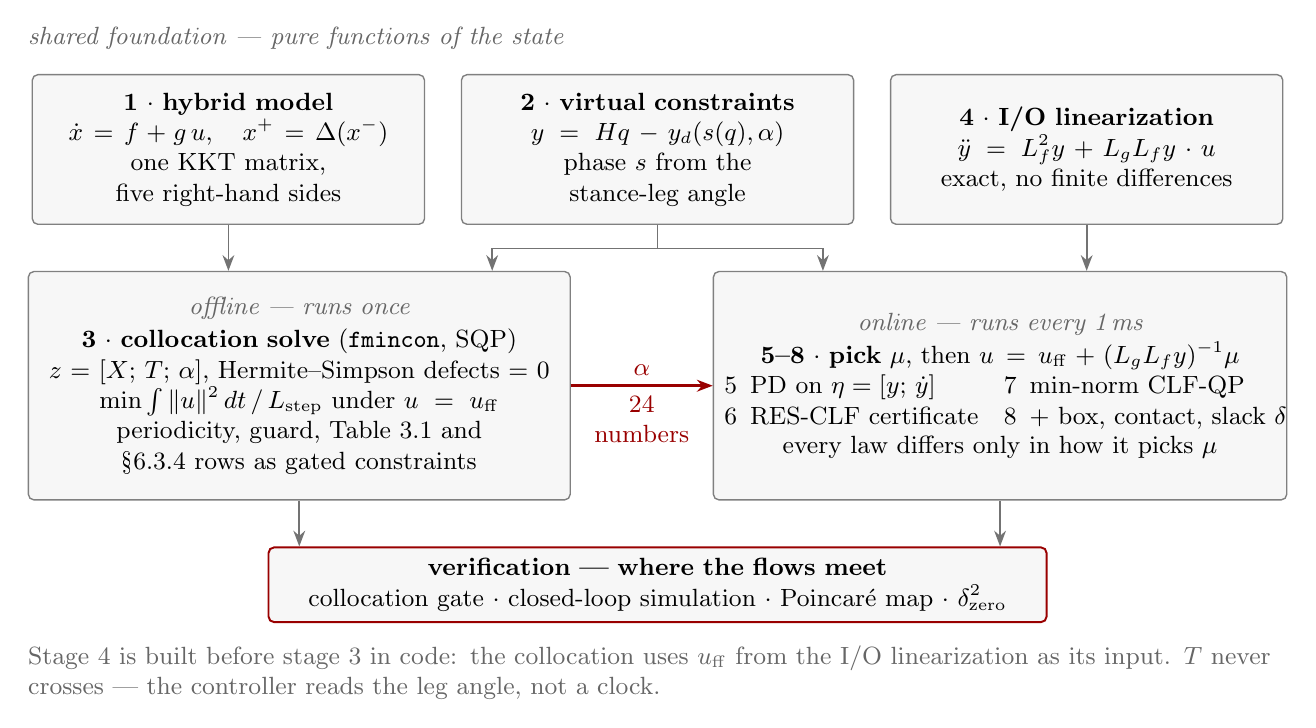
\begin{tikzpicture}[
        font=\small,
        box/.style={draw=black!50, fill=black!3, rounded corners=2pt, line width=0.5pt,
                    align=center, inner sep=4pt, anchor=north},
        arr/.style={-{Stealth[length=2mm]}, line width=0.6pt, draw=black!55},
        sub/.style={text=black!60}
    ]
    \node[anchor=south west, inner sep=0pt, sub] at (0,0)
        {\itshape shared foundation --- pure functions of the state};
    \node[box, text width=4.7cm, minimum height=1.9cm] (b1) at (2.55,-0.3)
        {\textbf{1 $\cdot$ hybrid model}\\ $\dot x = f + g\,u,\quad x^+ = \Delta(x^-)$\\
         one KKT matrix, five right-hand sides};
    \node[box, text width=4.7cm, minimum height=1.9cm] (b2) at (8.0,-0.3)
        {\textbf{2 $\cdot$ virtual constraints}\\ $y = Hq - y_d(s(q),\alpha)$\\
         phase $s$ from the stance-leg angle};
    \node[box, text width=4.7cm, minimum height=1.9cm] (b4) at (13.45,-0.3)
        {\textbf{4 $\cdot$ I/O linearization}\\ $\ddot y = L_f^2 y + L_gL_f y\cdot u$\\
         exact, no finite differences};
    \node[box, text width=6.6cm, minimum height=2.9cm] (b3) at (3.45,-2.8)
        {{\itshape\color{black!60} offline --- runs once}\\[1pt]
         \textbf{3 $\cdot$ collocation solve} (\texttt{fmincon}, SQP)\\
         $z = [X;\,T;\,\alpha]$, Hermite--Simpson defects $= 0$\\
         $\min \int \|u\|^2\,dt \,/\, L_{\mathrm{step}}$ under $u = u_{\mathrm{ff}}$\\
         periodicity, guard, Table~3.1 and \S6.3.4 rows as gated constraints};
    \node[box, text width=7.0cm, minimum height=2.9cm] (b58) at (12.35,-2.8)
        {{\itshape\color{black!60} online --- runs every 1\,ms}\\[1pt]
         \textbf{5--8 $\cdot$ pick $\mu$}, then $u = u_{\mathrm{ff}} + (L_gL_f y)^{-1}\mu$\\
         \begin{tabular}{@{}l@{\quad}l@{}}
           5\enspace PD on $\eta = [y;\,\dot y]$ & 7\enspace min-norm CLF-QP\\
           6\enspace RES-CLF certificate & 8\enspace + box, contact, slack $\delta$
         \end{tabular}\\
         every law differs only in how it picks $\mu$};
    \node[box, text width=9.6cm, draw=red!60!black, line width=0.7pt] (bv) at (8.0,-6.3)
        {\textbf{verification --- where the flows meet}\\
         collocation gate $\cdot$ closed-loop simulation $\cdot$
         Poincar\'e map $\cdot$ $\delta^2_{\mathrm{zero}}$};
    \draw[arr] (b1.south) -- (b1.south |- b3.north);
    \draw[arr] (b4.south) -- (b4.south |- b58.north);
    \draw[arr] (b2.south) -- ++(0,-0.3) -| (5.9,-2.8);
    \draw[arr] (b2.south) -- ++(0,-0.3) -| (10.1,-2.8);
    \draw[arr, draw=red!60!black, line width=0.9pt] (b3.east) -- (b58.west)
        node[midway, above, text=red!60!black] {$\alpha$}
        node[midway, below, align=center, text=red!60!black] {24\\numbers};
    \draw[arr] (b3.south) -- (b3.south |- bv.north);
    \draw[arr] (b58.south) -- (b58.south |- bv.north);
    \node[anchor=north west, text width=16cm, align=left, inner sep=0pt, sub] at (0,-7.55)
        {Stage 4 is built before stage 3 in code: the collocation uses $u_{\mathrm{ff}}$ from the
         I/O linearization as its input. $T$ never crosses --- the controller reads the leg angle,
         not a clock.};
    \end{tikzpicture}
    \end{latin}
    \caption{خط لوله فصل سوم. زیربنای مشترک (مدل هیبریدی، قیدهای مجازی و خطی‌سازی
    ورودی\nd{}خروجی) دو جریان را تغذیه می‌کند: حل هم‌محلی برون‌خط که یک بار اجرا می‌شود و
    $\alpha$ را تولید می‌کند، و قوانین کنترلی برخط که در هر میلی‌ثانیه اجرا می‌شوند. تنها
    $\alpha$ از جریان برون‌خط به برخط می‌رود. حل در زیر پیش‌خور محض و روی سطح دینامیک صفر
    $Z=\{\eta=0\}$ انجام می‌شود، جایی که هر جمله پس‌خوراند در صفر ضرب می‌شود. متن درون شکل انگلیسی است.}
    \label{fig:pipeline}
\end{figure*}

% =====================================================================
\section{مدل هیبریدی: یک ماتریس \en{KKT}، دو بار}
% =====================================================================
در فاز تک‌اتکا پای اتکا ثابت است و نگه‌داشتن آن به نیروی تماس $\lambda$ نیاز دارد. شتاب‌ها و
این نیرو از یک دستگاه نقطه‌زینی به دست می‌آیند:
\begin{equation}
\begin{bmatrix} M & -J_{\mathrm{st}}^{\top} \\ J_{\mathrm{st}} & 0 \end{bmatrix}
\begin{bmatrix} \ddot q \\ \lambda \end{bmatrix}
=
\begin{bmatrix} Bu - V - G \\ -\dot J_{\mathrm{st}}\dot q \end{bmatrix}
\label{eq:kkt}
\end{equation}
ماتریس سمت چپ شامل $u$ نیست، پس یک تجزیه با پنج سمت راست (یک رانش و چهار جهت ورودی)
وابستگی اَفین را دقیقاً بازیابی می‌کند:
\begin{equation}
\ddot q = \ddot q_{\mathrm{drift}} + \ddot q_{\mathrm{in}}\,u,\qquad
\lambda = \lambda_{\mathrm{drift}} + \lambda_{\mathrm{in}}\,u
\label{eq:affinesplit}
\end{equation}
این دقت، بنیان بقیه فصل است: مرحله $4$ ماتریس جداسازی دقیق را از $\ddot q_{\mathrm{in}}$
می‌سازد، و مرحله $8$ می‌تواند مخروط اصطکاک و کف نیروی عمودی را به صورت سطرهای \emph{خطی} در $u$
بنویسد، چون $\lambda$ نسبت به $u$ اَفین است. مجموعه آزمون $f+g\,u$ را با حل مستقیم \en{KKT}
($1.7\times10^{-13}$) و $\lambda$ را با آن ($1.3\times10^{-13}$) می‌سنجد.

برخورد پا همان ماتریس با معنایی دیگر است: موازنه تکانه به‌جای موازنه نیرو، که سرعت‌های پس از
برخورد و ضربه را حل می‌کند و با ژاکوبین پای نوسانی شرط $J_{\mathrm{sw}}\dot q^{+}=0$ را اعمال
می‌کند: پا فرود می‌آید و می‌چسبد ($6.7\times10^{-16}$). برچسب‌گذاری مجدد پاها \emph{پس از}
برخورد انجام می‌شود و نه پیش از آن؛ اگر ابتدا برچسب‌گذاری شود، $J_{\mathrm{sw}}$ پای اتکای
قبلی را توصیف می‌کند که شرط را از پیش برقرار می‌کند، پس ضربه دقیقاً صفر می‌شود و برخورد
بی‌صدا هیچ کاری نمی‌کند. جدول~\ref{tab:model} این مدل را در طول گام مرجع نشان می‌دهد.

\begin{table}[H]
    \centering
    \caption{مدل، اندازه‌گیری‌شده در طول گام مرجع ($61$ نقطه، مدل $74$ کیلوگرمی)}
    \label{tab:model}
    \small
    \begin{tabular}{lc}
        \toprule
        کمیت & مقدار \\
        \midrule
        جرم کل $M(1,1)$ & $74.000$ کیلوگرم \\
        عدد وضعیت ماتریس \en{KKT} & $896$ تا $1611$ \\
        $\mathrm{rcond}(L_gL_fy)$ & $4.5\times10^{-3}$ تا $1.0\times10^{-2}$ \\
        $\sigma_{\min}(L_gL_fy)$ (\en{HH2}) & $0.0862$ \\
        انرژی جنبشی در برخورد & $142.4$ به $99.1$ ژول \\
        ضربه $(I_x,\,I_z)$ & $(-5.59,\ 13.98)$ نیوتن‌ثانیه \\
        \bottomrule
    \end{tabular}
\end{table}

در هر برخورد $30.4$ درصد انرژی جنبشی در یک لحظه تلف می‌شود؛ این مهم‌ترین اغتشاش حلقه
هیبریدی است. اندازه ضربه $15.06$ نیوتن‌ثانیه است، عمدتاً عمودی و در لبه مخروط اصطکاک.

% =====================================================================
\section{قیدهای مجازی و خطی‌سازی ورودی\nd{}خروجی}
% =====================================================================
حرکت مطلوب با زاویه مطلق پای اتکا نمایه‌گذاری می‌شود:
\begin{equation}
\theta = q_T + q_1 + \tfrac12 q_2 = c\,q,\qquad
s = \frac{\theta-\theta^{-}}{\theta^{+}-\theta^{-}}
\label{eq:phase}
\end{equation}
با $\theta^{-}=-0.15$ و $\theta^{+}=0.30$ رادیان، پس $s$ در هر گام از $0$ به $1$ می‌رود و
پس‌خوراند حاصل مستقل از زمان است. خروجی‌ها $y = Hq - y_d(s(q),\alpha)$ با منحنی بزیه درجه
$5$ برای چهار مفصل عملگردار تعریف می‌شوند، پس $\alpha$ یک ماتریس $4\times6$ است.

دو جزئیات اهمیت دارد. نخست، $\theta$ نسبت به $q$ \emph{خطی} است، پس $\partial s/\partial q$
یک سطر ثابت است و $L_f^2y$ تنها یک جمله انحنا دارد و نه هسیان متغیر فاز. دوم، $s$ تنها بیرون
از بازه $[-0.5,\,1.5]$ محدود می‌شود و نه در $[0,\,1]$: هر گام در $s=0$ آغاز می‌شود و ممیز
شناور آن را در هر دو سمت صفر قرار می‌دهد، پس محدودکردن سخت در آنجا گاه‌به‌گاه $\dot s$ را صفر
و جمله‌ای از $\dot y$ را حذف می‌کرد.

خروجی‌ها درجه نسبی دو دارند و با جایگذاری تفکیک دقیق بخش پیش:
\begin{align}
\ddot y &= L_f^2 y + L_gL_f y\,u, \nonumber\\
u &= u_{\mathrm{ff}} + (L_gL_fy)^{-1}\mu,\quad
u_{\mathrm{ff}} = -(L_gL_fy)^{-1}L_f^2y
\label{eq:iolin}
\end{align}
که $\ddot y=\mu$ را نتیجه می‌دهد. مجموعه آزمون $\ddot y$ را در برابر مشتق جریان \emph{واقعی}
($1.5\times10^{-9}$) و حفظ $\ddot y=0$ توسط $u_{\mathrm{ff}}$ را ($1.1\times10^{-14}$) تصدیق
می‌کند. این خطی‌سازی \textbf{جزئی} است و به ضرورت: روی منیفلد تماس، فاز تک‌اتکا $10$ بعد دارد،
حالت عرضی $\eta=[y;\,\dot y]$ هشت بعد است، و دو بعد باقی دینامیک صفر در $(\theta,\dot\theta)$
است. پس‌خوراند مالک $\eta$ است و تنها انتخاب $\alpha$ آن دو بعد دیگر را شکل می‌دهد.

% =====================================================================
\section{بهینه‌سازی برون‌خط به روش هم‌محلی}
% =====================================================================
گام با هم‌محلی مستقیم \cite{betts2010practical} به دست می‌آید. با $h=T/(N-1)$ هر بازه یک
باقی‌مانده هرمیت-سیمپسون دارد و صفرکردن این باقی‌مانده‌ها \emph{همان} قید دینامیک است؛ هیچ
حل‌گر معادله دیفرانسیلی درون بهینه‌ساز نیست:
\begin{align}
x_m &= \tfrac12(x_k + x_{k+1}) + \tfrac{h}{8}(f_k - f_{k+1}), \nonumber\\
\zeta_k &= x_{k+1} - x_k - \tfrac{h}{6}(f_k + 4f_m + f_{k+1})
\label{eq:hs}
\end{align}
تابع هزینه $J = L_{\mathrm{step}}^{-1}\int_0^T \|u\|^2\,dt$ انرژی بر واحد مسافت است؛ بدون این
تقسیم، درجا زدن ارزان‌ترین گام می‌شد. بردار تصمیم $z=[X;\,T;\,\alpha]$ دارای $14N+25$ درایه
است: در $N=61$ گام مرجع، $879$ مجهول در برابر $869$ تساوی. $\alpha$ همان چیزی است که حل برای
آن انجام می‌شود و $854$ حالت نقطه‌ای تنها دینامیک را جبری می‌کنند. نامساوی‌ها در $18$ سطر
دروازه‌دار قرار دارند و سطری که دروازه‌اش خاموش است در $-1$ نگه داشته می‌شود و حذف نمی‌شود، تا
ابعاد مسئله میان شروع‌های گرم تغییر نکند.

\subsection{دروازه تأیید: باقی‌مانده کوچک به معنای مسیر واقعی نیست}
باقی‌مانده‌های برقرار یعنی معادلات \emph{گسسته} برقرارند. روی شبکه‌ای که برای دینامیک بیش از حد
درشت است، بهینه‌ساز به‌راحتی یک جواب گسسته جعلی برمی‌گرداند و هر عدد برگرفته از آن ساختگی است.
از این رو دروازه تأیید حلقه بسته را از نقطه نخست با \en{RelTol} برابر $10^{-11}$
انتگرال می‌گیرد و با حالت‌های نقطه‌ای مقایسه می‌کند؛ گامی که از آن بگذرد در این گزارش
\emph{تأییدشده} خوانده می‌شود. گام مرجع با $1.6\times10^{-4}$ (آستانه
$10^{-3}$) از این دروازه می‌گذرد و شبیه‌سازی رو به جلو زیر \en{PD} آن را بازتولید می‌کند:
$0.427$ متر در $0.273$ ثانیه در هر شش گام شبیه‌سازی‌شده.

\subsection{تبدیل مرتبه پنج است؛ پایه پیش‌فرض آن را نشان نمی‌دهد}
باقی‌مانده محلی هرمیت-سیمپسون باید مانند $h^5$ کاهش یابد. آزمون مرتبه روی مسیر بذر و روی
نردبان $N=9$ تا $33$ اجرا می‌شود. روی پایه بزیه درجه پنج\md{}پایه‌ای که همه گام‌های ذخیره‌شده،
از جمله گام مرجع، با آن حل شده‌اند\md{}مرتبه بیشینه باقی‌مانده $3.51$، $4.19$ و $4.51$ و میانه
آن $4.19$ است (ستون بزیه جدول~\ref{tab:order})، و آزمون الزامی مجموعه آزمون روی همین پایه
است. روی پایه پیش‌فرض (\en{B-spline} درجه سه) همان آزمون با میانه مرتبه $0.58$
\textbf{شکست} می‌خورد. این شکست واقعی است، اما از تبدیل نیست
(شکل~\ref{fig:order} و جدول~\ref{tab:order})، و به همین دلیل به‌عنوان شکست مورد انتظار
مستند نگه داشته می‌شود.

\begin{figure*}[t]
    \centering
    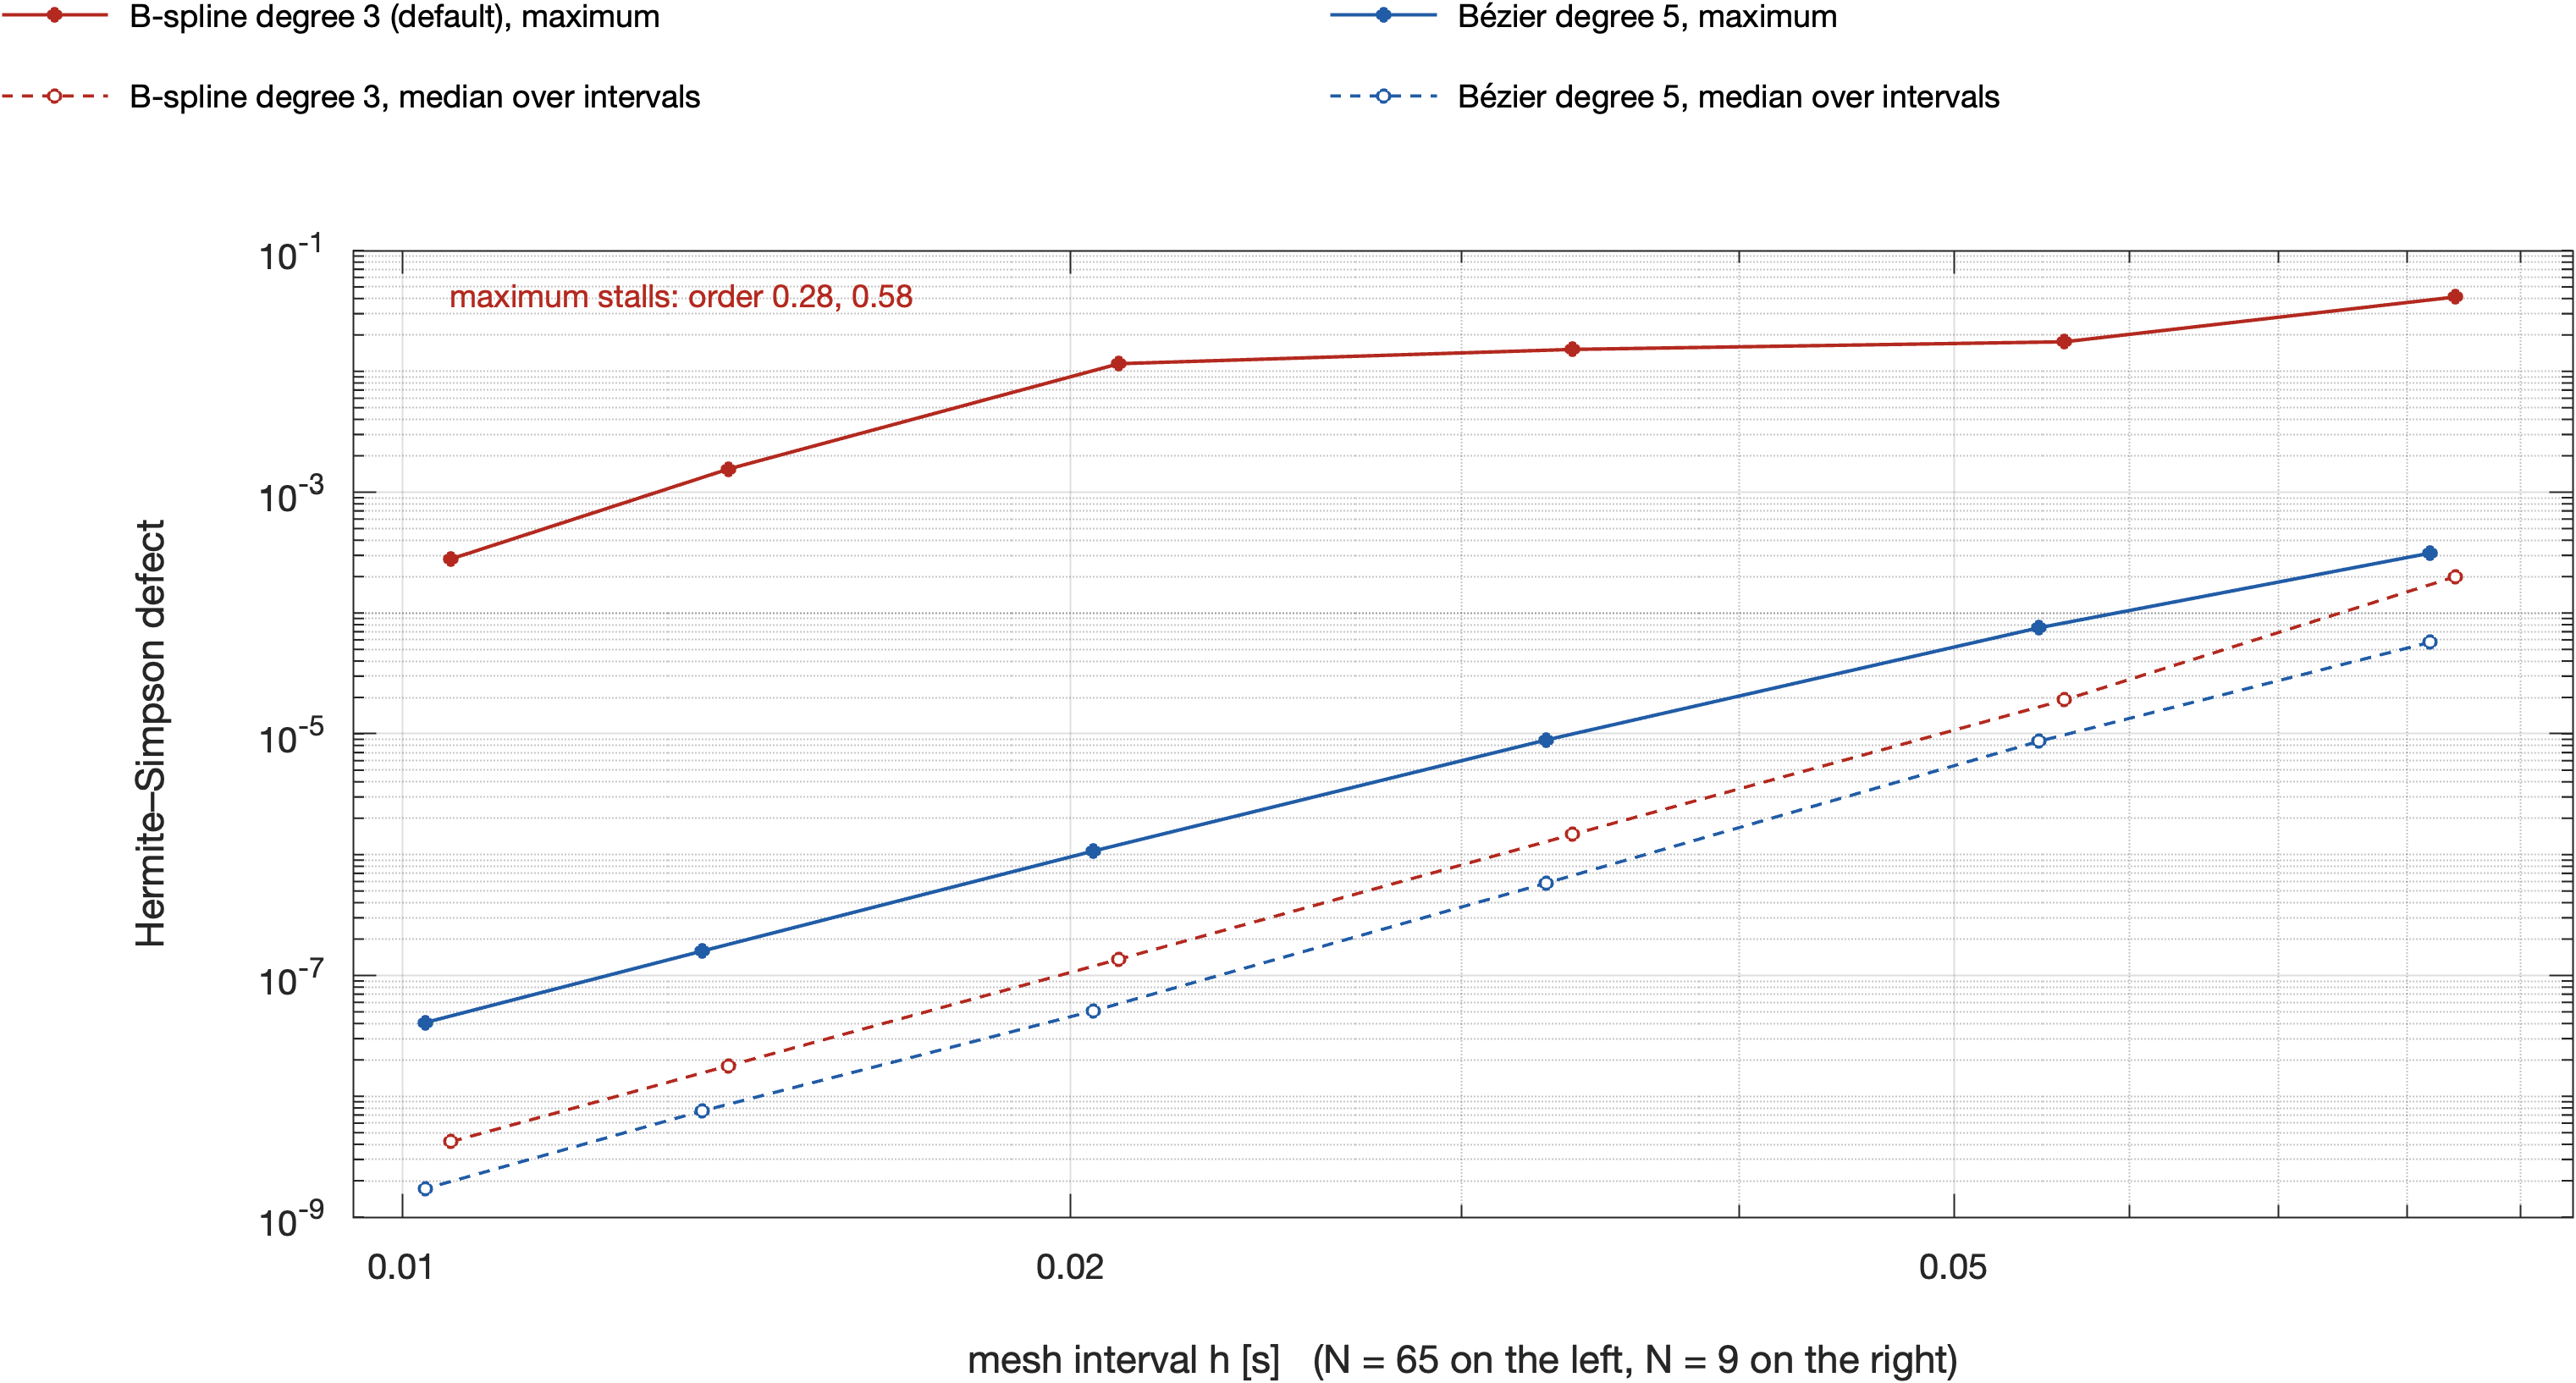
\includegraphics[width=0.82\textwidth]{ch3_defect_order.png}
    \caption{هم‌گرایی باقی‌مانده هرمیت-سیمپسون روی مدل $74$ کیلوگرمی. \emph{میانه} باقی‌مانده بازه‌ها
    برای هر دو پایه با مرتبه حدود پنج کاهش می‌یابد ($5.18$ و $5.00$ در کل پالایش): تبدیل درست است.
    \emph{بیشینه} در پایه \en{B-spline} درجه سه متوقف می‌شود. از $N=13$ به بعد این بیشینه در
    سطر سرعت زانوی پای نوسانی و در فاز $s\approx0.62$ تا $0.67$ قرار دارد و در $N=65$ در
    $0.33$، یعنی در گره‌های داخلی $1/3$ و $2/3$، جایی که $y_d$ تنها $C^2$ است.
    \en{B-spline} درجه پنج همان منحنی بزیه است و مقادیر یکسان دارد.}
    \label{fig:order}
\end{figure*}

\begin{table*}[!t]
    \centering
    \caption{بیشینه باقی‌مانده و مرتبه آن در پالایش شبکه، روی مسیر بذر}
    \label{tab:order}
    \small
    \begin{tabular}{lccccc}
        \toprule
        $N$ & \en{B-spline} درجه $3$: بیشینه & مرتبه & بزیه درجه $5$: بیشینه & مرتبه & نسبت \\
        \midrule
        $9$  & $4.13\times10^{-2}$ & \nd{} & $3.13\times10^{-4}$ & \nd{} & $132$ \\
        $13$ & $1.76\times10^{-2}$ & $2.11$ & $7.54\times10^{-5}$ & $3.51$ & $233$ \\
        $21$ & $1.52\times10^{-2}$ & $0.28$ & $8.90\times10^{-6}$ & $4.19$ & $1707$ \\
        $33$ & $1.16\times10^{-2}$ & $0.58$ & $1.07\times10^{-6}$ & $4.51$ & $10803$ \\
        $49$ & $1.55\times10^{-3}$ & $4.95$ & $1.59\times10^{-7}$ & $4.73$ & $9737$ \\
        $65$ & $2.80\times10^{-4}$ & $5.96$ & $4.07\times10^{-8}$ & $4.62$ & $6868$ \\
        \bottomrule
    \end{tabular}
\end{table*}

بیشینه \en{B-spline} به‌جای کُند بودن، نامنظم است: اندازه آن به محل افتادن هر گره درون بازه
بستگی دارد، پس مرتبه آن از $0.28$ تا $5.96$ می‌پرد. پیش‌فرض درجه سه به‌عنوان منحنی‌ای متفاوت از
بزیه و بررسی مستقلی بر اینکه خط لوله به پایه وابسته نیست نگه داشته شده است. آزمون مرتبه آن
شکست مورد انتظار ثبت می‌شود و مجموعه آزمون را شکست نمی‌دهد؛ اما اگر روزی \emph{بگذرد}، مجموعه
آزمون شکست می‌خورد، تا توضیح بالا بی‌صدا کهنه نشود. «مرتبه پنج» درباره \emph{میانه} باقی‌مانده
است؛ مرتبه \emph{بیشینه} با پایه بزیه در این پالایش از $4.73$ فراتر نمی‌رود.

\subsection{مجموعه قیدهای بخش \en{6.3.4} روی گام مرجع}
مجموعه کامل قیدهای بخش \en{6.3.4} کتاب \cite{westervelt2007feedback} به صورت سطرهای
دروازه‌دار پیاده شده است. هر کمیت در جدول~\ref{tab:set} اندازه‌گیری شده، چه دروازه‌اش هنگام حل
روشن بوده باشد چه نه؛ قاعده خط لوله «پیش از قیدگذاری اندازه بگیر» است.

\begin{table}[H]
    \centering
    \caption{گام مرجع در برابر حدود خودش؛ [\en{E}] یعنی اعمال‌شده در حل}
    \label{tab:set}
    \footnotesize
    \setlength{\tabcolsep}{4pt}
    \begin{tabular}{lccc}
        \toprule
        سطر & مقدار & حد & وضعیت \\
        \midrule
        \relax[\en{E}] بیشینه گشتاور & $195.0$ & $\le 195$ & فعال \\
        \relax[\en{E}] \en{NIC1} کمینه نیروی عمودی & $50.05$ & $\ge 50$ & نزدیک \\
        \relax[\en{E}] \en{NIC2} اصطکاک & $0.246$ & $\le 0.40$ & مجاز \\
        \relax[\en{E}] \en{NIC3} فاصله پای نوسانی & $0.0010$ & $\ge 0.0010$ & فعال \\
        \relax[\en{E}] \en{NIC3} سرعت برخورد & $-3.175$ & $\le -0.05$ & مجاز \\
        \relax[\en{E}] \en{NEC2} سرعت جداشدن پا & $0.0788$ & $\ge 0.01$ & مجاز \\
        \relax[\en{E}] \en{NEC3} نسبت ضربه & $0.4000$ & $\le 0.40$ & فعال \\
        \relax[\en{E}] \en{NEC4} $\zeta^*_2$ & $2.580$ & $\ge 0.136$ & مجاز \\
        \relax[\en{E}] \en{NEC5} $\delta^2_{\mathrm{zero}}$ & $0.7462$ & $\le 1$ & مجاز \\
        \relax[\en{E}] \en{HH6} کمینه $\dot\theta$ & $1.451$ & $\ge 0.10$ & مجاز \\
        \relax[\en{E}] زاویه تنه (درجه) & $+1.7$ تا $+4.5$ & $\ge +1.7$ & فعال \\
        \relax[\en{E}] ارتفاع لگن (متر) & $0.916$ تا $0.943$ & $0.925\pm0.045$ & مجاز \\
        \relax[\ ] ضربه برخورد & $15.06$ & $\le 15$ & تجاوز \\
        \relax[\ ] بیشینه ارتفاع پای نوسانی & $0.212$ & $\le 0.15$ & تجاوز \\
        \en{HH4/HH5} $|\eta(\Delta x_N)|$ & $7.5\times10^{-7}$ & \nd{} & ضمنی \\
        \bottomrule
    \end{tabular}
\end{table}

سه سطر قید هم‌زمان فعال‌اند، در محدوده تحمل $7\times10^{-6}$ نامساوی‌های حل؛ زاویه تنه روی کران
خود است و نیروی عمودی $0.05$ نیوتن بالای کف خود می‌ماند. ناوردایی هیبریدی
(\en{HH4/HH5}) سطری ندارد: نقطه نخست روی $Z$ قرار می‌گیرد و با $\Delta(x_N)$ برابر می‌شود، پس
ناوردایی ضمنی است و به‌جای فرض، اندازه‌گیری می‌شود. دو حدی که دروازه‌شان در این حل خاموش بود،
به اندازه $0.06$ نیوتن‌ثانیه و $6$ سانتی‌متر تجاوز شده‌اند. گام با سرعت $1.563$ متر بر ثانیه،
نوسان لگن $2.7$ سانتی‌متر و هزینه $16026$ راه می‌رود (شکل~\ref{fig:gait}).

\begin{figure*}[t]
    \centering
    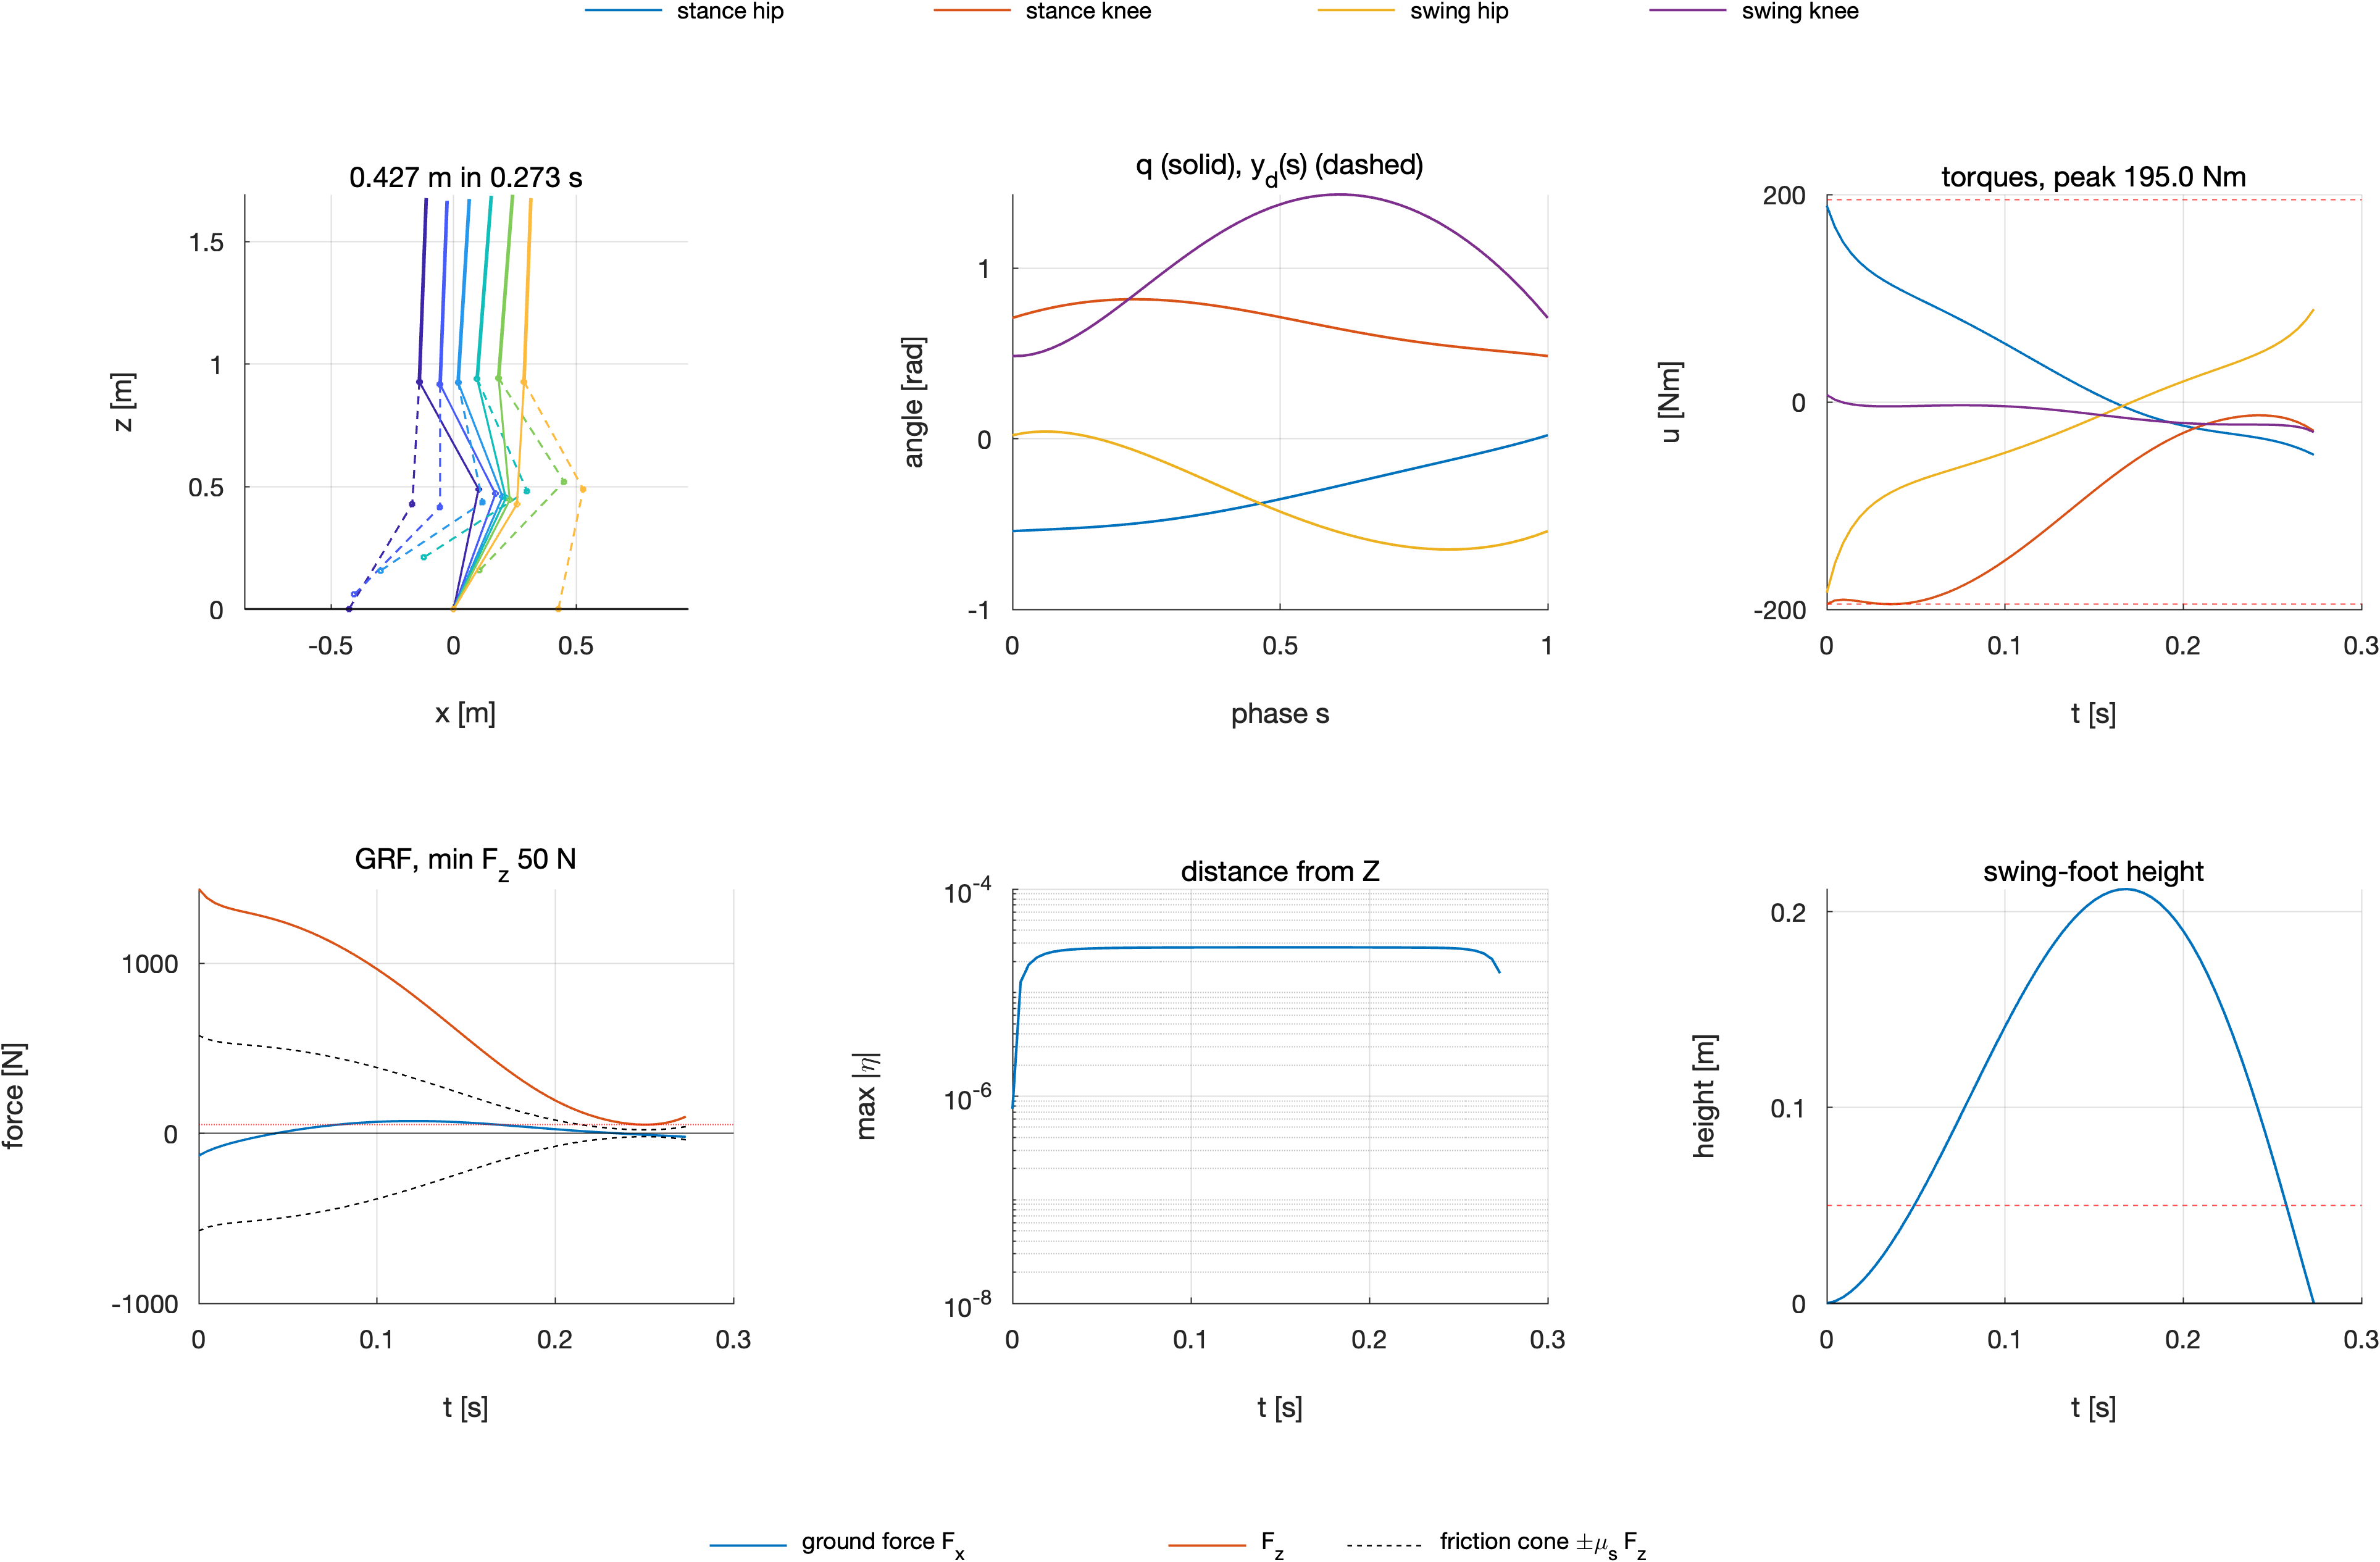
\includegraphics[width=\textwidth]{ch3_gait_posture195.png}
    \caption{گام مرجع. بالا: یک گام $0.427$ متری در $0.273$ ثانیه؛ زاویه مفاصل روی منحنی‌های
    بزیه؛ گشتاورها که در ابتدای گام به جعبه $\pm195$ نیوتن‌متر می‌رسند. پایین: نیروی عمودی که
    درست پیش از فرود به کف $50$ نیوتنی می‌رسد و درون مخروط اصطکاک می‌ماند؛ فاصله از $Z$ که
    تنها با پیش‌خور زیر $3\times10^{-5}$ می‌ماند؛ و ارتفاع پای نوسانی که در میانه گام از $0.05$
    متر می‌گذرد و به $0.21$ متر می‌رسد.}
    \label{fig:gait}
\end{figure*}

\subsection{شروع سرد روی این مدل گام نمی‌یابد؛ شروع گرم می‌یابد}
روند مستند، حل با حدود خاموش و سپس روشن‌کردن آن‌ها یکی‌یکی است: نیروی عمودی، اصطکاک، گشتاور
و ضربه، هر کدام با نردبانی که با شروع گرم پایین می‌آید. این روند از بذر تحلیلی روی مدل
$74$ کیلوگرمی هرگز به مسیر تأییدشده نمی‌رسد (جدول~\ref{tab:cold}).

\begin{table}[H]
    \centering
    \caption{نردبان از شروع سرد ($18$ حل، هر یک با دروازه تأیید سنجیده‌شده)}
    \label{tab:cold}
    \footnotesize
    \setlength{\tabcolsep}{4pt}
    \begin{tabular}{lccc}
        \toprule
        مرحله & انحراف & سرعت & بیشینه گشتاور \\
        \midrule
        بدون حد & $6.5$ & $0.134$ & $523$ \\
        + نیروی عمودی & $11.9$ & $0.137$ & $2334$ \\
        + اصطکاک & $16.7$ & $0.138$ & $2379$ \\
        گشتاور، پله $1$ تا $8$ & $7.6$ تا $32.6$ & $0.136$ تا $0.303$ & $298$ تا $1404$ \\
        گشتاور $9$ تا $12$، ضربه $1$ تا $3$ & $7.65$ & $0.148$ & $246$ \\
        \bottomrule
    \end{tabular}
\end{table}

آستانه تأیید $10^{-3}$ است و هیچ مرحله‌ای به سه مرتبه بزرگی آن نزدیک نمی‌شود. مدت گام‌ها روی
کران $1.5$ ثانیه می‌نشیند و از پله نهم گشتاور به بعد حل‌گر کاملاً می‌ایستد: هفت حل پیاپی نقطه
یکسانی برمی‌گردانند.

گام مرجع از راه دیگری به دست آمد (جدول~\ref{tab:warm}). بذر آن یک گام $61$ نقطه‌ای است که
روی نسخه $30$ کیلوگرمی همین هندسه (تنه $10$، هر ران و هر ساق $5$ کیلوگرم) حل شده بود. این بذر
در یک گام روی دینامیک $74$ کیلوگرمی هم‌گرا شد (انحراف $1.3\times10^{-5}$، سرعت $1.314$ متر
بر ثانیه، بیشینه گشتاور $287$ نیوتن‌متر) و سپس با نردبان‌های گشتاور به سوی حد
$120$ نیوتن‌متری پروژه پیش رفت.

\begin{table*}[!t]
    \centering
    \caption{مسیر رسیدن به گام مرجع؛ هر ردیف با دروازه تأیید سنجیده شده است}
    \label{tab:warm}
    \small
    \begin{tabular}{lccccc}
        \toprule
        مرحله & جعبه گشتاور & بیشینه گشتاور & انحراف & سرعت & نتیجه \\
        \midrule
        بذر هم‌گراشده روی مدل $74$ کیلوگرمی & خاموش & $287.0$ & $1.3\times10^{-5}$ & $1.314$ & تأییدشده \\
        نردبان $1$، پله‌های $1$ و $2$ & $281$ به $212$ & $281.3\;|\;211.7$ & $5.1\times10^{-4}\;|\;4.7\times10^{-4}$ & $1.526\;|\;1.549$ & تأییدشده \\
        نردبان $1$، پله‌های $3$، $4$ و ضربه & $159$ به $120$ & $164.8\;|\;148.2$ & $0.13$ تا $0.83$ & $1.54$ تا $1.70$ & رد: مسیر واقعی نیست \\
        نردبان $2$، پله $1$ & $195$ & $195.0$ & $4.4\times10^{-4}$ & $1.561$ & تأییدشده \\
        نردبان $2$، پله‌های $2$ تا $7$ & $180$ به $120$ & $123$ تا $240$ & $1.1$ تا $20$ & $0.29$ تا $1.50$ & رد: مسیر واقعی نیست \\
        وضعیت بدن، پله $1$ & $195$ & $195.0$ & $1.4\times10^{-4}$ & $1.537$ & تأییدشده \\
        وضعیت بدن، پله $2$ = گام مرجع & $195$ & $195.0$ & $1.6\times10^{-4}$ & $1.563$ & تأییدشده \\
        \bottomrule
    \end{tabular}
\end{table*}

این دو نردبان زیر $195$ نیوتن‌متر گام تأییدشده‌ای نمی‌یابند و گام حاصل جعبه $u_{\max}=195$
خودش را دارد، در برابر حد $120$ نیوتن‌متری که پروژه برای عملگرها اعلام کرده است. نردبان سومی
که \emph{پس از} یافتن گام اجرا می‌شود\md{}کاهش جعبه از یک گام $1.2$ متربرثانیه‌ای، با سرعت
آزاد\md{}تا $162.5$ نیوتن‌متر پایین می‌آید و همان‌جا متوقف می‌شود (بخش~\ref{sec:torquefloor}).

\textbf{حد $120$ نیوتن‌متر عدد جدول \en{3.1} نیست.} حدود جدول \en{3.1} اعداد ربات \en{ATRIAS}
هستند\md{}$63$ کیلوگرم با کاهنده $50:1$، پس $5$ نیوتن‌متر آن $250$ نیوتن‌متر در مفصل
است\md{}و به این مدل منتقل نمی‌شوند. \en{RABBIT} منتشرشده نیز رانش مستقیم ندارد: هر یک از
چهار مفصل آن با یک موتور، کاهنده هارمونیک $50:1$ و تسمه به حرکت درمی‌آید
\cite[جدول~I و شکل~4]{chevallereau2003rabbit}. در این مدل $u$ گشتاور \emph{سمت مفصل}، پس از
کاهنده، است؛ اینرسی بازتابیده روتور و اصطکاک کاهنده در آن مدل نشده‌اند. فصل چهارم هر دو را
در مجموعه عدم‌قطعیت ساختاریافته خود می‌آورد.

\textbf{ادامه روی پارامترهای مدل.} بذر از $30$ به $74$ کیلوگرم در \emph{یک} گام پریده است؛
پس معلوم نیست میان این دو ربات، خانواده گام‌هایی که در $120$ نیوتن‌متر جا می‌شوند کجا پایان
می‌یابد. چون $M$، $V$ و $G$ نسبت به جرم‌ها و اینرسی‌های لینک‌ها خطی‌اند و هندسه دو ربات یکی
است، ترکیب $(1-\lambda)$ برابر پارامترهای قدیم و $\lambda$ برابر پارامترهای جدید دقیقاً رباتی
میانی است. آزمایش ادامه، $\lambda$ را از $0$ تا $1$ با جعبه گشتاور ثابت $120$ نیوتن‌متر و با
شروع گرم از پله قبل پیش می‌برد؛ بذر آن گامی روی مدل $30$ کیلوگرمی است که هر چهار سطر جدول
\en{3.1} را در $120$ نیوتن‌متر برآورده می‌کند (بیشینه $120.0$ نیوتن‌متر، $0.975$ متر بر ثانیه).
جایی که دیگر گامی نمی‌یابد، $\lambda^*$، و سطرهای فعال پیش از آن ثبت می‌شوند؛ سپس از
$\lambda^*$ تا $1$ با جعبه خاموش ادامه می‌یابد تا گشتاور \emph{لازم} همین خانواده بر حسب جرم
خوانده شود. هر پله با دروازه تأیید سنجیده و با امضای مدل خودش ذخیره می‌شود. \textbf{نتیجه این
آزمایش هنوز اندازه‌گیری نشده است}؛ تا آن زمان، ادعای این گزارش تنها این است که روی مدل
$74$ کیلوگرمی، از این بذر و با نردبان‌های اجراشده، هیچ گام تأییدشده‌ای زیر $162.5$ نیوتن‌متر
یافت نشد.

% =====================================================================
\section{پایداری مداری: دو گواهی هم‌خوان}
% =====================================================================
قید تناوب، حالت آغاز گام را \emph{نقطه ثابت} نگاشت گام\nd{}به\nd{}گام می‌کند، و یک نقطه ثابت
می‌تواند دفع‌کننده باشد، هر قدر هم باقی‌مانده آن کوچک باشد. دو گواهی مستقل محاسبه می‌شود.
گواهی مستقیم نگاشت پوانکاره را در $13$ جهت (به‌جز $p_x$) با تفاضل مرکزی می‌سازد و شعاع طیفی
$\rho$ را برمی‌گرداند؛ این کار $26$ شبیه‌سازی گام هزینه دارد. گواهی غیرمستقیم دینامیک روی $Z$
را با تصویر روی بردار هم‌وردایی که هم عملگرها و هم نیروی تماس را صفر می‌کند، به معادله نرده‌ای
$a(\theta)\ddot\theta + b(\theta)\dot\theta^2 + c(\theta) = 0$ فرومی‌کاهد. یک عامل انتگرال‌ساز
نگاشت گام را نسبت به $\zeta=\sigma^2/2$ اَفین می‌کند، پس نقطه ثابت و مقدار ویژه آن تنها از
$\alpha$ و به شکل بسته به دست می‌آیند (جدول~\ref{tab:hzd}).

\begin{table}[H]
    \centering
    \caption{پایداری مداری گام مرجع}
    \label{tab:hzd}
    \small
    \begin{tabular}{lc}
        \toprule
        کمیت & مقدار \\
        \midrule
        شعاع طیفی پوانکاره $\rho$ ($26$ گام) & $0.7462$ \\
        $\delta^2_{\mathrm{zero}}$ (انتگرال روی $\alpha$) & $0.746156$ \\
        $\dot\theta^{-}$: پیش‌بینی $|$ هم‌محلی & $2.398819\;|\;2.398998$ \\
        $\zeta^{-}$: پیش‌بینی $|$ هم‌محلی & $2.579877\;|\;2.580263$ \\
        $\zeta^*_2$ در برابر $V_{\max}/\delta^2$ & $2.580\;|\;0.136$ \\
        شبیه‌سازی رو به جلو زیر \en{PD} & $6$ گام از $6$ \\
        \bottomrule
    \end{tabular}
\end{table}

$\rho$ و $\delta^2$ تا $5\times10^{-5}$ هم‌خوان‌اند و اختلاف نسبی نقطه ثابت $1.5\times10^{-4}$
است. $\delta^2$ مقدار ویژه دینامیک صفر است، پس $\rho$ نگاشت کامل نباید از آن کمتر شود، و نمی‌شود.
مجموعه آزمون کاهش مدل را در برابر مدل کامل $14$ حالته ($5.0\times10^{-10}$) و پایستگی
$\tfrac12\sigma^2 + V_{\mathrm{zero}}(\theta)$ را در طول یک شبیه‌سازی واقعی
($2.3\times10^{-6}$) تصدیق می‌کند؛ ناوردایی‌ای که اگر عامل انتگرال‌ساز نادرست باشد تصادفاً
برقرار نمی‌ماند. هر دو گواهی محلی‌اند: خطی‌سازی حول مدار را توصیف می‌کنند و ناحیه جذب را
کران‌دار نمی‌کنند.

% =====================================================================
\section{کنترل‌کننده‌ها: چهار راه انتخاب $\mu$}
% =====================================================================
همه کنترل‌کننده‌ها $L_f^2y$، $L_gL_fy$ و $u_{\mathrm{ff}}$ یکسانی دریافت می‌کنند و تنها در
انتخاب $\mu$ تفاوت دارند:
\textbf{\en{PD}} روی $\eta$ با $K_p=100$ و $K_d=20$؛
\textbf{\en{RES-CLF}} با $V=\eta^{\top}P_\varepsilon\eta$ و نرخ لازم
$\dot V\le-(c_3/\varepsilon)V$ \cite{ames2014resclf}، که از معادله \en{CARE} مقدار $c_3=0.366$
و از معادله لیاپانوف $0.381$ به دست می‌آید؛
\textbf{\en{CLF-QP}} کمینه‌نرم که کوچک‌ترین $\mu$ برقرارکننده این نرخ را به شکل بسته می‌دهد
(در برابر حل عددی با \en{quadprog}: $9.0\times10^{-11}$) و دقیقاً با نسبت $1.0000$ روی کران حرکت
می‌کند؛ و \textbf{\en{CLF-QP} قیددار} با جعبه گشتاور، سطرهای اصطکاک و نیروی عمودی\md{}خطی،
چون $\lambda$ نسبت به $u$ اَفین است\md{}و متغیر شل $\delta$ روی سطر \en{CLF} با جریمه
$10^{6}$، تا تعارض به‌جای ناشدنی‌کردن برنامه، نرخ را آزاد کند.

کنترل‌کننده قیددار باید به صورت \textbf{داده نمونه‌برداری‌شده} اجرا شود: $u(x)$ آن تنها
قطعه‌ای هموار است و در هر تغییر مجموعه فعال شکست دارد، و حل‌گر تطبیقی هر شکست را خطای ناموفق
می‌خواند و متوقف می‌شود. حل یک بار در هر میلی‌ثانیه و نگهداری گشتاور، انتگرال‌ده را درون هر
دوره هموار می‌کند؛ مجموعه آزمون مرتبه اول بودن خطای نگهدارنده را تصدیق می‌کند (نسبت‌های نصف‌شدن
$1.97$ و $2.00$).

مقایسه کنترل‌کننده‌ها روی گام مرجع، گام‌به‌گام اجرا شد: هر سه قانون با
نمونه‌برداری $1$ کیلوهرتز، چهار گام، با \en{CLF} خودِ گام (\en{CARE} و $\varepsilon=0.5$). تنها
کنترل‌کننده قیددار از جعبه گشتاور باخبر است؛ جعبه پیش‌فرض $60$ درصد بیشینه $195$ نیوتن‌متری گام
است و کنترل‌کننده قیددار در $80$ و $100$ درصد نیز اجرا شد. گامی که کوتاه‌تر از $0.15$ متر یا با
$\max\|\eta\|$ بیش از $10^3$ پایان یابد، سقوط شمرده می‌شود (جدول~\ref{tab:ctrl}).

\begin{table*}[!t]
    \centering
    \caption{کنترل‌کننده‌ها روی گام مرجع با نمونه‌برداری $1$ کیلوهرتز. ستون پنجم
    بیشینه $\|\eta\|$ در گام‌های پیاپی است؛ $\dagger$ گام سقوط را نشان می‌دهد. ستون
    «گام‌های معتبر» گام‌های کامل‌شده پیش از نخستین نمونه‌ای است که تماس را نقض می‌کند
    ($F_z\le0$ یا $|F_x|/F_z>0.4$).}
    \label{tab:ctrl}
    \small
    \begin{tabular}{lccccc}
        \toprule
        کنترل‌کننده & جعبه (نیوتن‌متر) & گام‌ها & گام‌های معتبر & بیشینه $\|\eta\|$ گام‌به‌گام & بیشینه گشتاور \\
        \midrule
        \en{PD} & بی‌خبر & $4$ از $4$ & $4$ & $0.107\leftarrow0.215\leftarrow0.214\leftarrow0.213$ & $195.2$ \\
        \en{CLF-QP} کمینه‌نرم & بی‌خبر & سقوط در $3$ & $1$ & $0.228\leftarrow2.44\leftarrow\dagger$ & $283.5$ \\
        \en{CLF-QP} قیددار & $117$ ($60$ درصد) & سقوط در $2$ & $0$ & $3.31\leftarrow\dagger$ & $117.0$ \\
        \en{CLF-QP} قیددار & $156$ ($80$ درصد) & سقوط در $2$ & $0$ & $0.859\leftarrow\dagger$ & $156.0$ \\
        \en{CLF-QP} قیددار & $195$ ($100$ درصد) & سقوط در $4$ & $1$ & $0.227\leftarrow2.41\leftarrow143\leftarrow\dagger$ & $195.0$ \\
        \bottomrule
    \end{tabular}
\end{table*}

کنترل‌کننده \en{PD} راه می‌رود و روی مدار خودش آرام می‌گیرد، هرچند از جعبه $117$ نیوتن‌متری
$78$ نیوتن‌متر فراتر می‌رود. پس «\en{PD} راه می‌رود» نتیجه‌ای است در افق چهار گام و بدون قید
گشتاور، و نه مقایسه‌ای با بودجه یکسان. \en{CLF-QP} بی‌قید خطا را در گام دوم ده برابر می‌کند و گام سوم
$0.42$ متر پشت نقطه آغازش پایان می‌یابد. نسخه قیددار جعبه را همیشه دقیقاً رعایت می‌کند: در
$60$ درصد، $\delta$ در گام نخست به $199$ می‌رسد؛ در $100$ درصد تا وقتی جعبه فعال نشده، همان
رفتار قانون بی‌قید را دارد و گام سوم به $\delta=4.8\times10^{5}$ و $94$ بار حل جایگزین نیاز
دارد. شبیه‌ساز فصل سوم خود تشخیص سقوط ندارد و گذر از سطح برخورد، گام را حتی وقتی ربات روی زمین
است پایان می‌دهد؛ به همین دلیل این مقایسه معیار سقوط بالا را به کار می‌برد.

\textbf{شمارش گام کافی نیست.} شبیه‌ساز پای اتکا را \textbf{لولا} می‌گیرد: نه بلند می‌شود و
نه می‌لغزد، هر چه کنترل‌کننده از زمین بخواهد. پس گامی که نیروی تماسش پا را به داخل زمین
می‌کشد ($F_z\le0$) یا اصطکاکی بیش از $\mu_s=0.4$ می‌طلبد، در شمارش گام‌ها «راه رفتن» به
حساب می‌آید. پس هر اجرا در برابر تماسی که فرض می‌کند سنجیده می‌شود: اجرا تا نخستین نمونه
نامعتبر \emph{معتبر} است، و هیچ گامی پس از آن نمونه در ستون «گام‌های معتبر» شمرده نمی‌شود.
شبیه‌ساز گزینه‌ای نیز دارد که در همان نمونه متوقف شود، تا اجرای طولانی چیزی را که روی زمین
واقعی رخ نمی‌داد شبیه‌سازی نکند. با این معیار تنها \en{PD}
هر چهار گام را معتبر راه می‌رود؛ \en{CLF-QP} بی‌قید در گام دوم می‌لغزد
($\max|F_x|/F_z=25$، $\min F_z=-883$ نیوتن) و نسخه قیددار در $60$ و $80$ درصد همان گام
نخست را نیز به پایان نمی‌رساند. بنابراین «سقوط در گام سوم» برای قانون بی‌قید، خوش‌بینانه
است: ربات واقعی پیش از آن از مدار خارج شده است.

\textbf{همین آزمون در $\varepsilon=0.20$.} برای آنکه هر سه فصل در یک نرخ نتیجه بگیرند،
جدول~\ref{tab:ctrl} در $\varepsilon=0.20$\md{}مقداری که فصل چهارم برمی‌گزیند\md{}نیز اجرا
شد: سقوط‌ها دیرتر رخ می‌دهند یا در افق چهار گام رخ نمی‌دهند\md{}کمینه‌نرم در گام $4$ به‌جای $3$؛ قیددار
در $60$ درصد همچنان در گام $2$، در $80$ درصد در گام $3$ به‌جای $2$، و در $100$ درصد در
چهار گام سقوط نمی‌کند\md{}اما شمار گام‌های معتبر دست‌نخورده می‌ماند ($4$، $1$، $0$، $0$،
$1$). در این دو مقدار، نتیجه این بخش به انتخاب $\varepsilon$ وابسته نیست.

\textbf{کمینه‌نرم بودن به معنای خوش‌رفتاری نیست.} \en{CLF-QP} بی‌قید دقیقاً همان هم‌گرایی را
می‌خواهد که \en{RES-CLF} تضمین می‌کند، و در $\varepsilon=0.5$ این مقدار زیاد نیست:
$c_3/\varepsilon=0.732$ ثابت زمانی $1.37$ ثانیه در برابر گام $0.273$ ثانیه‌ای است، پس برقراری
دقیق نرخ، $V$ را در هر گام تنها $18$ درصد کاهش می‌دهد ($e^{-0.732\times0.273}$). سپس برخورد
$\eta$ را برمی‌جهاند و تضمین فاز پیوسته درباره $\Delta$ چیزی نمی‌گوید. \en{PD} به این نرخ گره
نخورده است\md{}به‌طور گذرا از کران \en{CARE} فراتر می‌رود اما در کل بیشتر هم‌گرا می‌شود\md{}و روی
همان گام با $\max\|\eta\|=0.21$ آرام می‌گیرد. مازاد هم‌گرایی که بهینه‌سازی کمینه‌نرم چنین کارآمد
حذف می‌کند، همان چیزی است که هزینه پایداری در گذر از برخورد را می‌پرداخت. فصل چهارم از همین‌جا
آغاز می‌کند: پیش از هر اندازه‌گیری زیر خطای مدل، $\varepsilon$ را از $0.5$ به $0.20$ می‌کاهد.

\textbf{این توضیح یک فرضیه است و رقیبی اندازه‌گیری‌شده دارد.} دو داده با آن به‌تنهایی جور
درنمی‌آیند. نخست، $\varepsilon=0.20$ نرخ را $2.5$ برابر می‌کند (کاهش $39$ درصدی $V$ در هر
گام به‌جای $18$ درصد)، اما شمار گام‌های معتبر را تغییر نمی‌دهد. دوم، فصل چهارم با مدل
\emph{کامل} اندازه گرفته است که نگه‌داشتن ورودی در یک دوره نمونه به‌تنهایی، پس از نخستین
برخورد $\|\eta^+\|$ را به $0.242$ در $1$ میلی‌ثانیه، $0.123$ در $0.5$، $0.049$ در $0.2$ و
$1.7\times10^{-4}$ در کنترل پیوسته می‌رساند: خطایی متناسب با دوره نمونه که نگاشت برخورد آن
را بزرگ می‌کند. پس بخشی از آنچه در بالا به نرخ نسبت داده شد ممکن است اثر نمونه‌برداری
$1$ کیلوهرتز باشد. دو توضیح پیش‌بینی متفاوتی دارند: اگر نرخ مقصر باشد، کوتاه‌کردن دوره در
$\varepsilon$ ثابت چیزی را عوض نمی‌کند؛ اگر نمونه‌برداری مقصر باشد، قانون کمینه‌نرم با
کوتاه‌شدن دوره بهبود می‌یابد. آزمایش جداسازی، جدول~\ref{tab:ctrl} را در دوره‌های $1$،
$0.5$، $0.2$ و $0.1$ میلی‌ثانیه و در کنترل پیوسته، در هر دو $\varepsilon$، اجرا می‌کند و در هر
گام $\|\eta^-\|$ پیش از برخورد و $\|\eta^+\|$ پس از آن را ثبت می‌کند تا بزرگ‌نمایی برخورد از
خطای نگهدارنده جدا شود. \textbf{نتیجه آن هنوز اندازه‌گیری نشده است.}

\textbf{کران $\varepsilon$ از خودِ قضیه.} $\varepsilon$ در این فصل \emph{انتخاب} شده است؛
همان قضیه یک کران بالا نیز برای آن می‌دهد. میان دو برخورد
$V(T^-)\le e^{-c_3T/\varepsilon}\,V(0^+)$، و نزدیک نقطه ثابت برخورد $\eta$ را خطی می‌نگارد،
$\eta^+=J\eta^-$، پس
\begin{equation}
V(\eta^+)\le\gamma^2(\varepsilon)\,V(\eta^-),\quad
\gamma^2(\varepsilon)=\lambda_{\max}\!\left(J^{\top}P_\varepsilon J,\;P_\varepsilon\right),\quad
\rho_V(\varepsilon)=\gamma^2(\varepsilon)\,e^{-c_3T/\varepsilon}
\label{eq:epsbound}
\end{equation}
و \en{RES-CLF} حلقه هیبریدی را تنها جایی تضمین می‌کند که $\rho_V<1$. بزرگ‌ترین چنین
$\varepsilon$، یعنی $\varepsilon_{\max}$، کران بالای آن چیزی است که می‌تواند کار کند: کران در
زمان پیوسته و در خودِ نقطه ثابت است، و نمونه‌برداری و فاصله از مدار تنها وضع را بدتر می‌کنند.
صورت محافظه‌کارانه $\|J\|^2\,\mathrm{cond}(P_\varepsilon)\,e^{-c_3T/\varepsilon}$ نیز گزارش
می‌شود. $J$ در حالت پیش از برخورد نقطه ثابت گام مرجع و با تفاضل مرکزی از میان نگاشت برخورد،
با ثابت نگه‌داشتن مختصات دینامیک صفر، اندازه گرفته می‌شود. \textbf{مقدار $\varepsilon_{\max}$
هنوز اندازه‌گیری نشده است}؛ فاصله آن تا $0.5$ و $0.20$ همان عددی است که این بخش کم دارد.

% =====================================================================
\section{ملاحظات اندازه‌گیری‌شده}
% =====================================================================
\subsection{هر فایل گام باید مدلی را که روی آن حل شده ثبت کند}
توابع دینامیک تولیدشده ($M$، $V$ و $G$) سراسری‌اند. گامی که روی دینامیکی دیگر حل شده باشد
همچنان بارگذاری و شبیه‌سازی می‌شود، اما به‌عنوان مرجعی که مدار این ربات نیست
(جدول~\ref{tab:stale}).

\begin{table}[H]
    \centering
    \caption{گام‌های ذخیره‌شده، ارزیابی‌شده روی مدل $74$ کیلوگرمی. $\max|c_{\mathrm{eq}}|$
    بیشینه همه قیدهای تساوی حل است و انحراف، انحراف دروازه تأیید.}
    \label{tab:stale}
    \footnotesize
    \setlength{\tabcolsep}{4pt}
    \begin{tabular}{lccc}
        \toprule
        گام & $\max|c_{\mathrm{eq}}|$ & انحراف & وضعیت \\
        \midrule
        گام مرجع پیشین (\en{reference\_gait}) & $0.64$ & $0.76$ & مدار نیست \\
        \en{upright} & $0.69$ & $14$ & مدار نیست \\
        \en{lean\_tall\_nec3} & $0.47$ & $21$ & مدار نیست \\
        \en{fix} & $0.46$ & $56$ & مدار نیست \\
        \en{full\_constrained} & $0.34$ & $7.9$ & مدار نیست \\
        \en{fix\_reconverged} (بذر) & $1.2\times10^{-6}$ & $1.3\times10^{-5}$ & مدار \\
        گام مرجع & $7.6\times10^{-7}$ & $1.6\times10^{-4}$ & مدار \\
        \bottomrule
    \end{tabular}
\end{table}

پنج گام نخست روی مدل $30$ کیلوگرمی و دو گام آخر روی مدل $74$ کیلوگرمی حل شده‌اند. نخستین
گام جدول روی مدل $74$ کیلوگرمی نه‌تنها از مدارش خارج است بلکه ناپایدار است
($\delta^2_{\mathrm{zero}}=0.904$ و $\rho=1.180$)، و هیچ چیز در خودِ فایل‌ها این را نمی‌گفت.

از این رو هر حل هم‌محلی \emph{امضای مدل} خود را همراه گام ذخیره می‌کند: مقادیر $M$، $V$،
$G$ و سینماتیک پاها در سه حالت ثابت، از همان مدلی که حل روی آن انجام شده (برای مدل ترکیبی
بخش پیش، از همان ترکیب). هنگام بارگذاری، این امضا با مدلی که در مسیر است مقایسه می‌شود\md{}با
مقدار و تلورانس نسبی $10^{-9}$ و نه با چکیده، تا اختلاف رقم آخر میان دو ماشین آن را
نشکند\md{}و سه حکم ممکن است: \emph{هم‌خوان}؛ \emph{ناهم‌خوان}، یعنی گام روی دینامیکی دیگر حل
شده و هر عددی که از آن محاسبه شود درباره رباتی دیگر است؛ و \emph{ثبت‌نشده}، برای فایل‌هایی که
امضا ندارند. برای فایل ثبت‌نشده، بارگذار فصل چهارم همچنان گام را روی دینامیک موجود دوباره
ارزیابی می‌کند و گامی را که مدار نیست رد می‌کند؛ و ابزار مهاجرت تنها به گامی امضا می‌افزاید
که روی مدل موجود دوباره تأیید شود (تساوی‌ها زیر $10^{-4}$ و گذر از دروازه تأیید)، پس امضا
هرگز فایل کهنه‌ای را گواهی نمی‌کند. طبق جدول~\ref{tab:stale} تنها دو گام آخر این شرط را
دارند. \textbf{اجرای مهاجرت روی فایل‌های موجود هنوز انجام نشده است.}

\subsection{کف گشتاور این خانواده گام $162.5$ نیوتن‌متر است، نه $120$}
\label{sec:torquefloor}
حد اعلام‌شده پروژه $u_{\max}=120$ نیوتن‌متر است و گام مرجع با جعبه $195$ نیوتن‌متری خودش
حل شده است. اما $195$ کف این خانواده نیست: نردبانی که جعبه را از یک گام $1.2$
متربرثانیه‌ای، با سرعت آزاد، پایین می‌آورد چهار پله را فرود می‌آورد و پله آخر تمیز است
(جدول~\ref{tab:torquefloor}).

\begin{table}[H]
    \centering
    \caption{نردبان جعبه گشتاور از گام $1.2$ متربرثانیه‌ای، با سرعت آزاد. همه پله‌ها
    از دروازه تأیید گذشته‌اند؛ $\mu$ و کمینه نیروی عمودی در هر پله دقیقاً روی حد خود
    نشسته‌اند}
    \label{tab:torquefloor}
    \small
    \begin{tabular}{lccccc}
        \toprule
        جعبه (نیوتن‌متر) & سرعت & $\max|c|$ & انحراف تأیید & ضربه (نیوتن‌ثانیه) & حکم \\
        \midrule
        $180$   & $1.2815$ & $2.8\times10^{-6}$  & $3.2\times10^{-5}$ & $18.77$ & فرود \\
        $170$   & $1.2857$ & $6.3\times10^{-9}$  & $5.1\times10^{-5}$ & $18.88$ & فرود \\
        $165$   & $1.2935$ & $2.2\times10^{-6}$  & $6.3\times10^{-5}$ & $18.87$ & فرود \\
        $\mathbf{162.5}$ & $\mathbf{1.2921}$ & $\mathbf{7.3\times10^{-11}}$ & $\mathbf{7.1\times10^{-5}}$ & $19.07$ & \textbf{فرود تمیز} \\
        $160$   & \nd{} & $6.2\times10^{-4}$، $9.2\times10^{-4}$ & \nd{} & \nd{} & دو بار رد \\
        \bottomrule
    \end{tabular}
\end{table}

\textbf{و $162.5$ یک کف است، نه یک توقف.} آزمایش دیوار در $160$ نیوتن‌متر پنج
بار تلاش می‌کند و هر پنج بار رد می‌شود؛ مهم‌تر آنکه \emph{شل‌کردن قیدهای تماس کمکی نمی‌کند}:
با $\mu_s=0.5$ سطر گشتاور به $1.1\times10^{-2}$ و با کف نیروی عمودی $25$ نیوتن به
$1.3\times10^{-2}$ \emph{بدتر} می‌شود، چون بهینه‌ساز آزادی تازه را صرف خودِ تماس می‌کند
($\mu$ به $0.500$ و $F_z$ به $43.5$ می‌رود) و نه صرف گشتاور. پس مانع، مسیر است و نه هیچ‌یک
از حدها.

\textbf{سرعت در این شاخه برعکس شهود عمل می‌کند.} هرچه جعبه تنگ‌تر شد گام \emph{تندتر} شد
($1.2815$ به $1.2921$ متربرثانیه، با کوتاه‌شدن دوره گام و ثابت‌ماندن طول آن). طول ثابت
می‌ماند چون با $\theta^\pm$ ثابت، طول گام تنها از راه ارتفاع لگن در لحظه برخورد تغییر می‌کند
(بخش~\ref{sec:stridefixed})، و این ارتفاع در پله‌های فرودآمده تنها میان $0.9521$ و $0.9525$
متر است. پین‌کردن
سرعت روی $1.20$ حل را به یک جواب گسسته کاذب فرومی‌پاشد ($\max|c|=3.0$، انحراف تأیید
$1.2\times10^{-2}$). بنابراین $1.2$ متربرثانیه و $120$ نیوتن‌متر را نمی‌توان با ادامه همین
نردبان هم‌زمان دنبال کرد.

<<<<<<< Updated upstream
دو نکته باقی می‌ماند. نخست، $162.5$ هنوز $1.35$ برابر حد اعلام‌شده است؛ رسیدن به $120$ به
گامی \emph{دیگر} نیاز دارد (وضعیت بدن، طول گام یا شاخه سرعتِ دیگر) و نه به ادامه این نردبان.
دوم، ضربه این گام‌ها $18.8$ تا $19.1$ نیوتن‌ثانیه بود، بالاتر از حد $15$، چون دروازه آن در
همه این حل‌ها خاموش بود.

\textbf{این نکته دوم اکنون بسته شده است.} \code{ch3\_impulse\_march} گام $162.5$
نیوتن‌متری را برمی‌دارد، جعبه را نگه می‌دارد، دروازه ضربه را روشن می‌کند و سقف را با
پله‌های یک نیوتن‌ثانیه‌ای تا $15$ پایین می‌آورد، با سرعت آزاد (جدول~\ref{tab:impulsemarch}).
هر چهار پله فرود می‌آیند و پله آخر تمیز است: گامی با جعبه $162.5$ نیوتن‌متر و ضربه $15.00$
نیوتن‌ثانیه که همه حدهای اعمال‌شده را برآورده می‌کند ($\max c=-2.1\times10^{-9}$) و مسیر واقعی
است (انحراف تأیید $1.2\times10^{-4}$ در برابر آستانه $10^{-3}$). بهای آن باز هم سرعت است: گام
از $1.2921$ به $1.3932$ متربرثانیه تند می‌شود، $16$ درصد بالاتر از سرعت طراحی، با کوتاه‌شدن
دوره گام ($0.3395$ به $0.3144$ ثانیه) و ثابت‌ماندن طول آن ($0.438$ متر). با پایین آمدن ضربه،
تماس از گوشه خود جدا می‌شود: کف نیروی عمودی $50$ نیوتنی از $16$ نیوتن‌ثانیه به بعد فعال نیست
و در $15$ سطرهای فعال، گشتاور و ضربه‌اند.

\begin{table}[H]
    \centering
    \caption{نردبان ضربه از گام $162.5$ نیوتن‌متری، با جعبه ثابت و سرعت آزاد
    (\code{ch3\_impulse\_march}). همه پله‌ها مسیر واقعی‌اند. در پله $17$ تکرار نهایی حل
    حدها را برآورده نکرد و تکراری پیشین که همه را تا $6.3\times10^{-6}$ روی سطر اصطکاک برآورده
    می‌کرد نگه داشته شد؛ پله‌های پس از آن به‌تنهایی همه حدها را برآورده می‌کنند}
    \label{tab:impulsemarch}
    \small
    \begin{tabular}{lccccc}
        \toprule
        سقف ضربه & سرعت & کمینه $F_z$ & $\max c$ & انحراف تأیید & حکم \\
        \midrule
        $19.07$ (دانه) & $1.2921$ & $50.0$ & $7.3\times10^{-11}$ & $7.1\times10^{-5}$ & \nd{} \\
        $18$ & $1.3162$ & $50.0$ & $1.4\times10^{-10}$ & $9.6\times10^{-5}$ & فرود \\
        $17$ & $1.3460$ & $50.0$ & $6.3\times10^{-6}$ & $1.3\times10^{-4}$ & تکرار نگه‌داشته \\
        $16$ & $1.3707$ & $67.1$ & $<0$ & $1.4\times10^{-4}$ & فرود \\
        $\mathbf{15}$ & $\mathbf{1.3932}$ & $\mathbf{72.3}$ & $\mathbf{<0}$ & $\mathbf{1.2\times10^{-4}}$ & \textbf{فرود تمیز} \\
        \bottomrule
    \end{tabular}
\end{table}
=======
$162.5$ هنوز $1.35$ برابر حد اعلام‌شده است؛ رسیدن به $120$ به گامی \emph{دیگر} نیاز دارد
(وضعیت بدن، طول گام یا شاخه سرعتِ دیگر) و نه به ادامه این نردبان.
>>>>>>> Stashed changes

\textbf{در همین جعبه، ضربه به $15$ نیوتن‌ثانیه می‌رسد.} ضربه پله‌های بالا $18.8$ تا $19.1$
نیوتن‌ثانیه بود، بالاتر از حد $15$، چون دروازه آن در این حل‌ها خاموش بود. نردبان ضربه، از
پله $162.5$ و با همان جعبه، حد ضربه را با پله‌های $1$ نیوتن‌ثانیه‌ای پایین می‌آورد و به
$15.00$ می‌رسد (جدول~\ref{tab:impulse}): گامی تأییدشده که هر چهار سطر جدول \en{3.1}\md{}گشتاور
در جعبه $162.5$، اصطکاک، کف نیروی عمودی و ضربه\md{}را هم‌زمان برآورده می‌کند. هزینه آن سرعت
است: با طول گام ثابت $0.438$ متر، هر پله دوره گام را کوتاه‌تر کرد. این گام دو حد را همچنان
نقض می‌کند\md{}گشتاور $162.5$ در برابر $120$ نیوتن‌متر، و ارتفاع پای نوسانی $0.32$ متر در
برابر $0.15$، که دروازه‌اش در این نردبان خاموش بود\md{}و پایداری مداری آن اندازه‌گیری نشده است.
فصل‌های چهارم تا ششم همچنان روی گام مرجع اجرا می‌شوند.

\begin{table}[H]
    \centering
    \caption{نردبان ضربه در جعبه $162.5$ نیوتن‌متری. همه پله‌ها از دروازه تأیید گذشته‌اند؛
    $\max|c|$ بیشینه نقض نامساوی‌ها در واحد واقعی است}
    \label{tab:impulse}
    \small
    \begin{tabular}{lccccc}
        \toprule
        حد ضربه & سرعت & دوره گام & کمینه $F_z$ & $\max|c|$ & انحراف تأیید \\
        \midrule
        بذر ($19.07$) & $1.2921$ & $0.3395$ & $50.0$ & $7.3\times10^{-11}$ & $7.1\times10^{-5}$ \\
        $18$ & $1.3162$ & $0.3332$ & $50.0$ & $1.4\times10^{-10}$ & $9.6\times10^{-5}$ \\
        $17$ & $1.3460$ & $0.3258$ & $50.0$ & $6.3\times10^{-6}$ & $1.3\times10^{-4}$ \\
        $16$ & $1.3707$ & $0.3198$ & $67.1$ & $<0$ & $1.4\times10^{-4}$ \\
        $\mathbf{15}$ & $\mathbf{1.3932}$ & $\mathbf{0.3144}$ & $\mathbf{72.3}$ & $<0$ & $\mathbf{1.2\times10^{-4}}$ \\
        \bottomrule
    \end{tabular}
\end{table}

\subsection{با $\theta^\pm$ ثابت، طول گام تقریباً تعیین شده است}
\label{sec:stridefixed}
اگر راه‌رفتن آهسته روی گام بلند به تماس فشار می‌آورد، راه طبیعی این است که گام را
\emph{کوتاه} کنیم: پای اتکا کمتر کشیده می‌شود، پس $F_z$ بالاتر می‌ماند و اصطکاک کمتری
لازم است. این راه در این تبدیل تقریباً بسته است، و دلیلش هندسی است.

\textbf{اتحاد طول گام.} با ران و ساق $0.5$ متری، $\theta=q_T+q_1+\tfrac12q_2$ دقیقاً جهت
خط لگن تا پای اتکا نسبت به قائم است. در لحظه برخورد هر دو پا روی زمین‌اند، پای اتکا در
$\theta^+$ است و پای فرودآینده\md{}که پس از برچسب‌گذاری مجدد گام بعد را از $\theta^-$ آغاز
می‌کند\md{}در $\theta^-$. پس
\begin{equation}
L_{\mathrm{step}} = h_{\mathrm{imp}}\left(\tan\theta^+ - \tan\theta^-\right)
\label{eq:stride}
\end{equation}
که $h_{\mathrm{imp}}$ ارتفاع لگن در لحظه برخورد است (استخراج در پیوست~\ref{app:stride}).
همه گام‌های ذخیره‌شده این اتحاد را تا حدود $10^{-7}$ برآورده می‌کنند. با $\theta^\pm$ ثابت،
تنها اهرم باقی‌مانده $h_{\mathrm{imp}}$ است، و نوار ارتفاع لگن ($0.880$ تا $0.970$ متر) کفی
برای طول گام می‌گذارد: $L_{\mathrm{step}}\ge0.880\times0.4605=0.4052$ متر.

\textbf{آزمون.} سطر $19$ (سقف طول گام، دروازه‌دار و به‌صورت پیش‌فرض خاموش) برای آزمودن
کوتاه‌کردن گام به کار رفت. نتیجه یک‌دست بود: \textbf{طول گام حتی یک میلی‌متر هم کوتاه
نمی‌شود.} در هر اجرا نقض قید دقیقاً ثابت می‌ماند، تساوی‌ها برقرارند، گام حدود $10^{-5}$ متر
جابه‌جا می‌شود و سپس اندازه گام حل‌گر به $10^{-8}$ فرومی‌ریزد. آنچه آزموده شد:

\begin{itemize}\renewcommand{\labelitemi}{\lr{\textbullet}}
    \item \textbf{دو گام آغازین}: گام $1.2$ متربرثانیه‌ای (که $\mu$، $F_z$ و گشتاورش
          هر سه دقیقاً فعال‌اند) و گام مرجع (که حاشیه اصطکاک $0.155$ دارد).
          هر دو یکسان متوقف شدند، پس «گوشه فعال» توضیح آن نیست.
    \item \textbf{چهار اندازه پله}: سقف‌های $0.40$، $0.43$، و کاهش‌های $1$ و
          $0.1$ میلی‌متری. نقض کوچک‌تر کمکی نکرد.
    \item \textbf{هر دو تابع هدف}: گشتاور دوم بر واحد مسافت، و گشتاور دوم به‌تنهایی.
          تابع هدف مانع نبود.
    \item \textbf{مقیاس تابع هدف}: ضرب در $10^{-4}$ تا شدنی‌بودن در تابع شایستگی غالب
          شود. گام دقیقاً همان $1.3\times10^{-5}$ متر حرکت کرد.
    \item \textbf{مقیاس‌بندی مسئله}: با مقیاس‌بندی خودکار حل‌گر خاموش، حل به جواب گسسته
          کاذب واگرا می‌شود (انحراف $36$ از مسیر واقعی).
\end{itemize}

\textbf{آنچه اتحاد توضیح می‌دهد و آنچه نمی‌دهد.} پله $0.40$ متری زیر کف $0.4052$ است، پس از
آغاز ناشدنی بود. اما پله $0.43$ و کاهش‌های $1$ و $0.1$ میلی‌متری بالای کف‌اند: برای گام
$1.2$ متربرثانیه‌ای ($L=0.4385$، $h_{\mathrm{imp}}=0.952$) پله $0.43$ تنها
$h_{\mathrm{imp}}=0.934$ می‌خواهد که درون نوار است. پس اتحاد، توقف در آن پله‌ها را توضیح
نمی‌دهد. دو آزمایش برای آن آماده است. نخست، در خودِ نقطه‌ای که حل متوقف شد، رتبه ژاکوبین
قیدهای فعال (با و بدون سطر طول گام، با سطرهای تجمیع‌شده به تفکیک نقطه) و یک برنامه خطی
الاستیک اندازه گرفته می‌شود که می‌پرسد آیا \emph{هیچ} جهت مرتبه اولی هست که همه تساوی‌ها و
نامساوی‌های فعال را نگه دارد و گام را یک میلی‌متر کوتاه کند؛ اگر نیست، ضرایب برنامه خطی
قیدهای مانع را سطربه‌سطر نام می‌برند. دوم، تبدیل گزینه‌ای نیز دارد که $\theta^-$ و
$\theta^+$ را متغیر تصمیم می‌کند (درون $[-0.40,\,-0.02]$ و $[0.10,\,0.50]$ رادیان)، و همان
نردبان طول گام با آن تکرار می‌شود. \textbf{نتیجه هر دو هنوز اندازه‌گیری نشده است.}

پس در این تبدیل و با $\theta^\pm$ ثابت، طول گام \emph{خروجی} ارتفاع لگن در برخورد است و نه
متغیری که بتوان با آن معامله کرد. این گزاره‌ای درباره \emph{این} صورت‌بندی و این حل‌گر است و
نه اثباتی بر ناممکن‌بودن گام کوتاه: پارامترسازی دیگر\md{}بازه فاز آزاد یا کوتاه‌تر، شاخه
وضعیت بدن دیگر، یا حل سردی که از آغاز حول گام کوتاه ساخته شود\md{}ممکن است چنین گامی بیابد.

\subsection{پایه پیش‌فرض دقت را هزینه می‌کند}
پایه \en{B-spline} درجه سه بیشینه باقی‌مانده را در شبکه‌های کاربردی سه تا چهار مرتبه بزرگی بالاتر
از پایه بزیه نگه می‌دارد؛ به همین دلیل همه گام‌های ذخیره‌شده با پایه بزیه حل شده‌اند و آزمون
الزامی مرتبه روی همان پایه است.

% =====================================================================
\section{اعتبارسنجی نرم‌افزاری}
% =====================================================================
هر مرحله در برابر یک مرجع \emph{مستقل} سنجیده می‌شود و نه در برابر خودش
(جدول~\ref{tab:tests}). آخرین اجرای اندازه‌گیری‌شده مجموعه آزمون $83$ بررسی داشت: $82$ قبول
و یک \emph{شکست مورد انتظار}، آزمون مرتبه روی پایه \en{B-spline} درجه سه (میانه مرتبه
$0.58$)، در $6.4$ ثانیه. مجموعه افزون بر این‌ها $19$ بررسی دارد که هنوز اجرا نشده‌اند:
دوازده در پیمانه مدل (مدل ترکیبی، که در $\lambda=1$ بیت‌به‌بیت همان مدل $74$ کیلوگرمی، در
$\lambda=0$ همان مدل $30$ کیلوگرمی و در میانه میانگین آن دو و همچنان متقارن و مثبت معین است؛
و امضای مدل، که سه حکم هم‌خوان، ناهم‌خوان و ثبت‌نشده را از هم جدا می‌کند)، چهار در هم‌محلی
(آزمون مرتبه الزامی روی پایه بزیه جدا از شکست مورد انتظار، و بسته‌بندی $\theta^\pm$ آزاد)، و سه
در شبیه‌سازی (توقف درست در نخستین نمونه تماس نامعتبر، همان نمونه‌ای که سنجه اعتبار می‌یابد).

\begin{table}[H]
    \centering
    \caption{مجموعه آزمون فصل سوم: آخرین اجرای اندازه‌گیری‌شده ($83$ بررسی، $6.4$ ثانیه)
    و بررسی‌هایی که هنوز اجرا نشده‌اند}
    \label{tab:tests}
    \small
    \begin{tabular}{lccc}
        \toprule
        پیمانه & بررسی & نتیجه & اجرانشده \\
        \midrule
        ارتقای پارامترهای ذخیره‌شده & $16$ & قبول & \nd{} \\
        مدل: \en{KKT}، برخورد، سطح برخورد & $10$ & قبول & $12$ \\
        قیدهای مجازی و $\ddot y$ & $12$ & قبول & \nd{} \\
        کنترل‌کننده‌ها و گواهی‌ها & $13$ & قبول & \nd{} \\
        هم‌محلی & $4$ & $3$ قبول، $1$ مورد انتظار & $4$ \\
        شبیه‌سازی و نگهدارنده & $11$ & قبول & $3$ \\
        دینامیک صفر هیبریدی & $17$ & قبول & \nd{} \\
        \midrule
        \textbf{مجموع} & $\mathbf{83}$ & $\mathbf{82}$ قبول & $\mathbf{19}$ \\
        \bottomrule
    \end{tabular}
\end{table}

آزمون دینامیک صفر روی گام مرجع اجرا می‌شود و پیش از هر مقایسه بررسی می‌کند که این گام مدار
دینامیک موجود باشد ($7.6\times10^{-7}$)؛ سپس $\delta^2_{\mathrm{zero}}=0.74619$ با
$\rho=0.74621$ هم‌خوان است. این آزمون انتگرال را با $321$ نقطه می‌گیرد؛ مقدار $0.746156$
جدول~\ref{tab:hzd} از شبکه $161$ نقطه‌ای گزارش است.

% =====================================================================
\section{ادعاها و وضعیت آن‌ها}
% =====================================================================
جدول~\ref{tab:claims3} هر ادعای این گزارش را با شاهد آن و وضعیتش کنار هم می‌گذارد.
«اندازه‌گیری‌شده» یعنی عدد از اجرایی است که خروجی‌اش در جدول بازتولید
(پیوست~\ref{app:repro}) نام برده شده؛ «در انتظار اجرا» یعنی آزمایش نوشته شده اما هنوز
اجرا نشده، و گزارش تا آن زمان چیزی درباره نتیجه‌اش ادعا نمی‌کند.

\begin{table*}[!t]
    \centering
    \caption{ادعاهای فصل سوم}
    \label{tab:claims3}
    \small
    \begin{tabular}{p{0.33\textwidth}p{0.43\textwidth}p{0.14\textwidth}}
        \toprule
        ادعا & شاهد & وضعیت \\
        \midrule
        گام مرجع مداری تناوبی و پایدار از مدل $74$ کیلوگرمی است &
            دروازه تأیید $1.6\times10^{-4}$؛ $\rho=0.7462$ و $\delta^2=0.746156$؛ شش گام زیر \en{PD} &
            اندازه‌گیری‌شده \\
        گام مرجع سه حد خودش را نقض می‌کند &
            گشتاور $195$ در برابر $120$، ضربه $15.06$ در برابر $15$، ارتفاع پای نوسانی $0.212$ در برابر $0.15$ &
            اندازه‌گیری‌شده \\
        تبدیل هرمیت\nd{}سیمپسون روی پایه بزیه مرتبه بالا دارد &
            میانه مرتبه بیشینه باقی‌مانده $4.19$ روی نردبان $N=9$ تا $33$؛ مرتبه باقی‌مانده میانه حدود پنج &
            اندازه‌گیری‌شده؛ آزمون الزامی اجرانشده \\
        شروع سرد روی این مدل گام تأییدشده نمی‌یابد &
            $18$ حل، انحراف $6.5$ تا $32.6$ در برابر آستانه $10^{-3}$ &
            اندازه‌گیری‌شده \\
        کف گشتاور این خانواده $162.5$ نیوتن‌متر است &
            چهار پله فرود؛ $160$ پنج بار رد؛ شل‌کردن $\mu_s$ و کف $F_z$ آن را بدتر می‌کند &
            اندازه‌گیری‌شده \\
        در جعبه $162.5$ گامی تأییدشده هر چهار سطر جدول \en{3.1} را برآورده می‌کند &
            نردبان ضربه تا $15.00$ نیوتن‌ثانیه، $1.393$ متر بر ثانیه؛ ارتفاع پای نوسانی $0.32$ متر؛ پایداری اندازه‌گیری‌نشده &
            اندازه‌گیری‌شده \\
        خانواده $120$ نیوتن‌متری میان $30$ و $74$ کیلوگرم کجا پایان می‌یابد &
            ادامه روی ترکیب مدل $\lambda$ &
            در انتظار اجرا \\
        با $\theta^\pm$ ثابت، $L_{\mathrm{step}}=h_{\mathrm{imp}}(\tan\theta^+-\tan\theta^-)$ &
            همه گام‌های ذخیره‌شده تا حدود $10^{-7}$؛ کف $0.4052$ متر زیر پله $0.40$ &
            اندازه‌گیری‌شده \\
        چه چیز کوتاه‌شدن گام را بالای کف می‌بندد &
            رتبه قیدهای فعال و برنامه خطی الاستیک در نقطه توقف؛ نردبان با $\theta^\pm$ آزاد &
            در انتظار اجرا \\
        روی گام مرجع \en{PD} چهار گام معتبر راه می‌رود و \en{CLF-QP} کمینه‌نرم سقوط می‌کند &
            جدول~\ref{tab:ctrl} در $\varepsilon=0.5$ و $0.20$ &
            اندازه‌گیری‌شده \\
        سقوط \en{CLF-QP} از نرخ کند است و نه از نمونه‌برداری &
            جاروب دوره کنترل $1$ تا $0.1$ میلی‌ثانیه و کنترل پیوسته &
            فرضیه؛ در انتظار اجرا \\
        $\varepsilon_{\max}$ که \en{RES-CLF} با آن از برخورد می‌گذرد &
            رابطه~\eqref{eq:epsbound} در نقطه ثابت گام مرجع &
            در انتظار اجرا \\
        هر فایل گام مدلی را که روی آن حل شده ثبت می‌کند &
            امضای مدل و سه حکم؛ مهاجرت فایل‌های موجود &
            پیاده‌سازی‌شده؛ آزمون و مهاجرت اجرانشده \\
        \bottomrule
    \end{tabular}
\end{table*}

% =====================================================================
\section{نتیجه‌گیری}
% =====================================================================
<<<<<<< Updated upstream
خط لوله فصل سوم روی مدل امروزی \en{RABBIT} یک گام تناوبی، معتبر و پایدار با سرعت $1.563$ متر بر
ثانیه ارائه می‌دهد که دو گواهی مستقل پایداری آن تا چهار رقم هم‌خوان‌اند و روی سه قید فیزیکی
هم‌زمان قرار دارد. سه یافته مهم‌تر از این گام‌اند. نخست، فایل گام دینامیک حل خود را ثبت نمی‌کند
و همه گام‌های پیش از بازتولید مدل اکنون مرجع‌هایی نادرست‌اند. دوم، حل از شروع سرد روی مدل
$74$ کیلوگرمی گام نمی‌یابد؛ اما شروع گرم می‌یابد، و نردبان جعبه گشتاور از گام مرجع تا
$162.5$ نیوتن‌متر پایین می‌آید و همان‌جا می‌ایستد\md{}نه به دلیل اصطکاک یا کف نیروی عمودی، که
شل‌کردنشان وضع را بدتر می‌کند، بلکه به دلیل خودِ مسیر (بخش~\ref{sec:torquefloor}). حد
اعلام‌شده $120$ نیوتن‌متر با این خانواده گام سازگار نیست، اما در $162.5$ ضربه را هم می‌توان
به حد $15$ نیوتن‌ثانیه رساند، در $1.39$ متربرثانیه. سوم، \en{CLF-QP}
کمینه‌نرم با $\varepsilon=0.5$ و نمونه‌برداری $1$ کیلوهرتز روی این گام سقوط می‌کند، در حالی که
\en{PD} راه می‌رود؛ کنترل‌کننده قیددار آنچه مرحله $8$ وعده می‌دهد را انجام می‌دهد\md{}گشتاور هرگز از
جعبه خارج نمی‌شود و $\delta$ تعارض را آشکار گزارش می‌کند\md{}اما هسته آن همان قانون کمینه‌نرم است.
=======
خط لوله فصل سوم روی مدل $74$ کیلوگرمی یک گام تناوبی، تأییدشده و پایدار با سرعت $1.563$ متر
بر ثانیه ارائه می‌دهد که دو گواهی مستقل پایداری آن تا چهار رقم هم‌خوان‌اند و روی سه قید
فیزیکی هم‌زمان قرار دارد. همین گام سه حد مشخصات خودش را نقض می‌کند، و این نقض‌ها همان‌قدر
بخشی از نتیجه‌اند که پایداری آن.
>>>>>>> Stashed changes

رشته‌ای که فصل را به هم می‌بندد این است: \emph{تضمینی که در زمان پیوسته اثبات شده، در
پیاده‌سازیِ نمونه‌برداری‌شده با گشتاور محدود و تماس محدود دوام نمی‌آورد\md{}و هر تضمین تنها
آنچه را می‌پوشاند که در آن نوشته شده است.} سه مشاهده این را در این فصل نشان می‌دهند. نخست،
\en{CLF-QP} کمینه‌نرم با تضمین همگرایی در زمان پیوسته، با نمونه‌برداری $1$ کیلوهرتز سقوط
می‌کند و \en{PD} بی‌تضمین راه می‌رود؛ سهم نرخ کند و سهم نمونه‌برداری هنوز از هم جدا نشده
است. دوم، شبیه‌ساز پای اتکا را لولا می‌گیرد، پس «چهار گام کامل» درباره زمین واقعی چیزی
نمی‌گوید تا وقتی تماس در سنجه نوشته شود: با آن، تنها \en{PD} هر چهار گام را معتبر راه می‌رود.
سوم، فایل گام نمی‌گوید درباره کدام ربات است تا وقتی مدلش در آن نوشته شود؛ از این رو هر حل
امضای مدل خود را ذخیره می‌کند.

حدود این خانواده گام نیز اندازه‌گیری شده‌اند: کف گشتاور $162.5$ نیوتن‌متر، که شل‌کردن
قیدهای تماس آن را پایین نمی‌آورد؛ در همان جعبه، گامی تأییدشده که حد ضربه را نیز برآورده می‌کند؛
و طول گامی که با $\theta^\pm$ ثابت تقریباً تعیین شده است. حد اعلام‌شده $120$ نیوتن‌متر با این
خانواده سازگار نیست. آنچه به فصل چهارم \cite{nguyen2017thesis} می‌رسد: گام مرجع، تفکیک اَفین
دقیق که به تفکیک مدل واقعی و اسمی تبدیل می‌شود، حلقه نمونه‌برداری‌شده $1$ کیلوهرتز، و کاهش
$\varepsilon$ به $0.20$ به‌عنوان نخستین تصمیم طراحی. سه محدودیت همراه این نتایج می‌ماند: همه
گام‌های تأییدشده روی این مدل از یک بذر شروع گرم می‌آیند؛ گواهی‌های پایداری محلی‌اند و برخورد
در هر گام $30$ درصد انرژی جنبشی را تلف می‌کند؛ و جعبه $195$ نیوتن‌متری پایین‌ترین جعبه‌ای
است که گام مرجع با آن تأیید شد، نه مشخصه یک عملگر.

% ---------------------- مراجع ----------------------
\begin{LTR}
\printbibliography[title={مراجع}]
\end{LTR}


% =====================================================================
% پیوست: استخراج روابط
% =====================================================================
\onecolumn
\setcounter{section}{0}
\renewcommand{\thesection}{پ}
\renewcommand{\thesubsection}{پ-\arabic{subsection}}
\section{استخراج روابط}
\label{app:deriv}
این پیوست هر رابطه متن را گام‌به‌گام به دست می‌آورد و ترتیب آن همان ترتیب متن است.
نمادگذاری: $q\in\mathbb{R}^7$ مختصات تعمیم‌یافته (دو مختصه پایه شناور، زاویه تنه و چهار
مفصل)، $x=(q,\dot q)$، $M(q)$ ماتریس جرم، $V(q,\dot q)$ جملات کوریولیس و گریز از مرکز،
$G(q)$ گرانش، و $B=\begin{bmatrix}0_{3\times4}\\ I_4\end{bmatrix}$ ماتریس ورود گشتاورها.

% ---------------------------------------------------------------------
\subsection{دستگاه \en{KKT} فاز اتکا (رابطه~\eqref{eq:kkt})}
معادله لاگرانژ با نیروی تماس $\lambda$ که از طریق ژاکوبین پای اتکا وارد می‌شود:
\begin{equation*}
    M\ddot q+V+G=Bu+J_{\mathrm{st}}^{\top}\lambda .
\end{equation*}
پای اتکا ثابت است: $p_{\mathrm{st}}(q)=\text{ثابت}$. یک بار مشتق
$J_{\mathrm{st}}\dot q=0$ و بار دوم
\begin{equation*}
    J_{\mathrm{st}}\ddot q+\dot J_{\mathrm{st}}\dot q=0 .
\end{equation*}
این دو معادله را کنار هم بنویسید و جمله $\lambda$ را به سمت چپ ببرید:
\begin{equation*}
    \begin{bmatrix} M & -J_{\mathrm{st}}^{\top} \\ J_{\mathrm{st}} & 0 \end{bmatrix}
    \begin{bmatrix} \ddot q \\ \lambda \end{bmatrix}
    =\begin{bmatrix} Bu - V - G \\ -\dot J_{\mathrm{st}}\dot q \end{bmatrix}.
\end{equation*}

\textbf{تفکیک اَفین (رابطه~\eqref{eq:affinesplit}).} نام ماتریس سمت چپ را $K$ بگذارید؛ $K$ به
$u$ وابسته نیست و سمت راست نسبت به $u$ خطی است:
\begin{equation*}
    \begin{bmatrix} Bu-V-G \\ -\dot J_{\mathrm{st}}\dot q\end{bmatrix}
    =\underbrace{\begin{bmatrix} -V-G \\ -\dot J_{\mathrm{st}}\dot q\end{bmatrix}}_{r_0}
    +\sum_{j=1}^{4}\underbrace{\begin{bmatrix} B e_j \\ 0\end{bmatrix}}_{r_j}u_j .
\end{equation*}
چون $K^{-1}$ خطی است، $K^{-1}r_0$ رانش و $K^{-1}r_j$ ستون $j$ام ورودی را می‌دهد:
$\ddot q=\ddot q_{\mathrm{drift}}+\ddot q_{\mathrm{in}}u$ و
$\lambda=\lambda_{\mathrm{drift}}+\lambda_{\mathrm{in}}u$، بدون هیچ تقریبی. به همین دلیل
سطرهای اصطکاک $|\lambda_x|\le\mu_s\lambda_z$ و کف نیرو $\lambda_z\ge F_{\min}$ در $u$ خطی‌اند.

% ---------------------------------------------------------------------
\subsection{نگاشت برخورد}
برخورد آنی است: $q$ پیوسته می‌ماند و تنها سرعت‌ها می‌پرند. معادله حرکت را روی بازه
$[t^-,t^+]$ به طول صفر انتگرال بگیرید؛ جملات کران‌دار ($V$، $G$، $Bu$) سهمی ندارند و تنها
نیروی ضربه‌ای پای فرودآمده می‌ماند، با ضربه $I=\int F\,dt$:
\begin{equation*}
    M(\dot q^{+}-\dot q^{-})=J_{\mathrm{sw}}^{\top}I .
\end{equation*}
با شرط چسبیدن پا، $J_{\mathrm{sw}}\dot q^{+}=0$، همان ماتریس \en{KKT} با سمت راست دیگری به دست
می‌آید:
\begin{equation*}
    \begin{bmatrix} M & -J_{\mathrm{sw}}^{\top} \\ J_{\mathrm{sw}} & 0 \end{bmatrix}
    \begin{bmatrix} \dot q^{+} \\ I \end{bmatrix}
    =\begin{bmatrix} M\dot q^{-} \\ 0 \end{bmatrix}.
\end{equation*}
این نگاشت نسبت به $\dot q^{-}$ \emph{خطی} است (در بخش پ-۷ به کار می‌آید). اعداد جدول مدل:
اتلاف انرژی $1-99.1/142.4=0.304$، اندازه ضربه $\sqrt{5.59^2+13.98^2}=15.06$ و نسبت اصطکاک
$5.59/13.98=0.40$، یعنی درست روی لبه مخروط.

% ---------------------------------------------------------------------
\subsection{متغیر فاز و خطی‌سازی ورودی\nd{}خروجی (روابط~\eqref{eq:phase} و \eqref{eq:iolin})}
با $\Delta\theta=\theta^{+}-\theta^{-}$ و $\theta=c\,q$، مشتق $s$ نسبت به $q$ سطر ثابت
$c/\Delta\theta$ است. خروجی $y=Hq-y_d(s)$ را مشتق بگیرید:
\begin{equation*}
    \dot y=\Big(H-y_d'(s)\,\frac{c}{\Delta\theta}\Big)\dot q=:J_y\,\dot q,
    \qquad \dot s=\frac{c\,\dot q}{\Delta\theta}.
\end{equation*}
در مشتق دوم، چون $c$ ثابت است، تنها $y_d'$ با زمان تغییر می‌کند:
\begin{equation*}
    \ddot y=J_y\ddot q-y_d''(s)\,\dot s\,\frac{c\,\dot q}{\Delta\theta}
    =J_y\ddot q-y_d''(s)\,\dot s^{2}.
\end{equation*}
این همان «تنها یک جمله انحنا» است: اگر $\theta$ در $q$ غیرخطی بود، هسیان $\partial^2 s/\partial q^2$
نیز ظاهر می‌شد. با جای‌گذاری تفکیک اَفین:
\begin{equation*}
    \ddot y=\underbrace{J_y\ddot q_{\mathrm{drift}}-y_d''\dot s^{2}}_{L_f^2y}
    +\underbrace{J_y\ddot q_{\mathrm{in}}}_{L_gL_fy}\,u .
\end{equation*}
با $u=-(L_gL_fy)^{-1}L_f^2y+(L_gL_fy)^{-1}\mu$ جمله اول دقیقاً حذف می‌شود و $\ddot y=\mu$.

\textbf{شمارش ابعاد.} حالت $14$ بعد دارد؛ تماس دو مختصه و دو سرعت را قید می‌کند، پس
$14-4=10$. خروجی چهار مؤلفه دارد و $\eta=(y,\dot y)$ هشت بعد، پس $10-8=2$ بعد برای دینامیک صفر
$(\theta,\dot\theta)$ می‌ماند.

% ---------------------------------------------------------------------
\subsection{هم‌محلی هرمیت\nd{}سیمپسون (رابطه~\eqref{eq:hs})}
\textbf{نقطه میانی.} روی بازه $[t_k,t_k+h]$ چندجمله‌ای درجه سه $p(\tau)$ را طوری بسازید که
مقدار و شیب دو سر را تطبیق دهد: $p(0)=x_k$، $p'(0)=f_k$، $p(h)=x_{k+1}$، $p'(h)=f_{k+1}$.
توابع پایه هرمیت در $\tau=h/2$ مقادیر $\tfrac12$، $\tfrac12$، $\tfrac{h}{8}$ و $-\tfrac{h}{8}$ دارند، پس
\begin{equation*}
    x_m=p(h/2)=\tfrac12(x_k+x_{k+1})+\tfrac{h}{8}(f_k-f_{k+1}),\qquad f_m=f(x_m,u_m).
\end{equation*}

\textbf{باقی‌مانده.} دینامیک به صورت انتگرالی
$x_{k+1}-x_k=\int_{t_k}^{t_k+h}f\,dt$ است. انتگرال را با قاعده سیمپسون روی سه نقطه تقریب بزنید
و تفاضل را صفر کنید:
\begin{equation*}
    \zeta_k=x_{k+1}-x_k-\tfrac{h}{6}(f_k+4f_m+f_{k+1})=0 .
\end{equation*}
($\zeta_k$ اینجا باقی‌مانده است و به $\zeta$ دینامیک صفر در بخش پ-۷ ربطی ندارد.)

\textbf{چرا مرتبه پنج.} خطای قاعده سیمپسون $-\tfrac{h^5}{2880}f^{(4)}$ است و خطای درون‌یابی
هرمیت در $x_m$ از مرتبه $h^4$، که با ضریب $\tfrac{4h}{6}\,\partial f/\partial x$ وارد می‌شود و آن
هم $O(h^5)$ است. پس باقی‌مانده محلی روی یک مسیر هموار مانند $h^5$ کاهش می‌یابد. این برآورد به
$f^{(4)}$ کران‌دار نیاز دارد؛ \en{B-spline} درجه سه در گره‌های داخلی تنها $C^2$ است، مشتق‌های
بالاتر $y_d$ در آنجا می‌پرند، و بیشینه باقی‌مانده دقیقاً در همان فازها متوقف می‌شود.

\textbf{شمارش مجهول‌ها.} هر نقطه $14$ حالت دارد، به‌علاوه مدت گام $T$ و $4\times6=24$ ضریب
$\alpha$: $14N+1+24=14N+25$، که در $N=61$ برابر $879$ است.

% ---------------------------------------------------------------------
\subsection{\en{RES-CLF} و ثابت $c_3$}
بعد از خطی‌سازی، $\dot\eta=F\eta+G\mu$ با
$F=\begin{bmatrix}0&I\\0&0\end{bmatrix}$ و $G=\begin{bmatrix}0\\I\end{bmatrix}$.
تغییر مقیاس $\xi=I_\varepsilon\eta=(y/\varepsilon,\ \dot y)$ را تعریف کنید. آنگاه
\begin{equation*}
    \dot\xi=\begin{bmatrix}\dot y/\varepsilon\\ \mu\end{bmatrix}
    =\frac1\varepsilon\big(F\xi+G\,v\big),\qquad v:=\varepsilon\mu ,
\end{equation*}
یعنی همان انتگرال‌گیر دوگانه، $1/\varepsilon$ بار تندتر. با $V_\varepsilon=\xi^{\top}P\xi=\eta^{\top}P_\varepsilon\eta$
و $P_\varepsilon=I_\varepsilon PI_\varepsilon$:
\begin{equation*}
    \dot V_\varepsilon=\frac1\varepsilon\Big(\xi^{\top}(F^{\top}P+PF)\xi+2\xi^{\top}PG\,v\Big).
\end{equation*}
معادله \en{CARE} می‌گوید $F^{\top}P+PF=PGG^{\top}P-Q$. با انتخاب $v=-G^{\top}P\xi$:
\begin{equation*}
    \dot V_\varepsilon=\frac1\varepsilon\Big(-\xi^{\top}Q\xi-\|G^{\top}P\xi\|^2\Big)
    \le-\frac{\lambda_{\min}(Q)}{\varepsilon}\|\xi\|^2
    \le-\frac{1}{\varepsilon}\,\underbrace{\frac{\lambda_{\min}(Q)}{\lambda_{\max}(P)}}_{c_3}\,V_\varepsilon ,
\end{equation*}
زیرا $V_\varepsilon\le\lambda_{\max}(P)\|\xi\|^2$. پس دست‌کم یک $\mu$ شرط
$\dot V_\varepsilon\le-(c_3/\varepsilon)V_\varepsilon$ را برقرار می‌کند و مجموعه مجاز هیچ‌گاه خالی نیست.
به‌ویژه در $L_gV=0$ (یعنی $G^{\top}P\xi=0$) شرط بدون هیچ کنترلی برقرار است.

\textbf{کران نمایی.} از
$\lambda_{\min}(P)\|\xi\|^2\le V_\varepsilon\le\lambda_{\max}(P)\|\xi\|^2$ و
$\dot V_\varepsilon\le-(c_3/\varepsilon)V_\varepsilon$ داریم $V_\varepsilon(t)\le e^{-c_3t/\varepsilon}V_\varepsilon(0)$.
برای $\varepsilon<1$، $\|\eta\|\le\|\xi\|\le\|\eta\|/\varepsilon$، پس
\begin{equation*}
    \|\eta(t)\|\le\frac1\varepsilon\sqrt{\frac{\lambda_{\max}(P)}{\lambda_{\min}(P)}}\;e^{-c_3t/(2\varepsilon)}\;\|\eta(0)\| .
\end{equation*}

\textbf{نسخه لیاپانوف.} با \en{PD}، $\mu=-K_py-K_d\dot y$ و ماتریس حلقه‌بسته
$A=\begin{bmatrix}0&I\\-K_p&-K_d\end{bmatrix}$. اگر $A^{\top}P+PA=-Q$، همان استدلال بدون جمله
$\|G^{\top}P\xi\|^2$ تکرار می‌شود. قانون \en{PD} شرط کاهش را برقرار می‌کند، اما هیچ قضیه‌ای
تضمین نمی‌کند که در $L_gV=0$ نیز برقرار بماند.

% ---------------------------------------------------------------------
\subsection{\en{CLF-QP} کمینه‌نرم و کاهش $18$ درصدی}
با $\psi=L_fV+(c_3/\varepsilon)V$، شرط به صورت
$\psi+L_gV\,\mu\le0$ است. اگر $\psi\le0$، $\mu=0$ کافی است. در غیر این صورت کوچک‌ترین
$\mu$ تصویر مبدأ روی ابرصفحه $L_gV\,\mu=-\psi$ است:
\begin{equation*}
    \mu^*=-\frac{\psi}{\|L_gV\|^2}\,L_gV^{\top},
\end{equation*}
(لاگرانژ: $2\mu+\lambda L_gV^{\top}=0$ با قید فعال). روی این جواب
$\dot V=-(c_3/\varepsilon)V$ دقیقاً برقرار است، که همان نسبت $1.0000$ متن است.

\textbf{کاهش در یک گام.} با برقراری دقیق نرخ،
$V(T)=e^{-(c_3/\varepsilon)T}V(0)$. در $\varepsilon=0.5$ و $c_3=0.366$:
$c_3/\varepsilon=0.732$ و $e^{-0.732\times0.273}=e^{-0.200}=0.82$؛ یعنی $V$ در هر گام تنها
$18$ درصد کم می‌شود، و ثابت زمانی $1/0.732=1.37$ ثانیه است.

\textbf{خطای نگهدارنده.} با نگهداری $u_k$ در $[t_k,t_k+T_s]$،
$u(t)-u_k=\dot u\,(t-t_k)+O(T_s^2)$، پس انحراف مسیر از حالت پیوسته $O(T_s)$ است. نصف کردن
$T_s$ خطا را نصف می‌کند: نسبت $2$.

% ---------------------------------------------------------------------
\subsection{دینامیک صفر، عامل انتگرال‌ساز و نگاشت پوانکاره}
\textbf{معادله نرده‌ای.} روی $Z$ داریم $y=0$ و $\dot y=0$، پس $q=q_z(\theta)$ و
$\dot q=v_z(\theta)\dot\theta$، و در نتیجه
$\ddot q=v_z\ddot\theta+v_z'\dot\theta^2$. معادله حرکت را در سطری $w$ ضرب کنید که
$wB=0$ و $wJ_{\mathrm{st}}^{\top}=0$؛ گشتاورها و نیروی تماس حذف می‌شوند:
\begin{equation*}
    \underbrace{w\,M v_z}_{a(\theta)}\ddot\theta
    +\underbrace{w\big(M v_z'+V(q_z,v_z)\big)}_{b(\theta)}\dot\theta^2
    +\underbrace{w\,G(q_z)}_{c(\theta)}=0 ,
\end{equation*}
زیرا $V(q,\dot q)$ نسبت به $\dot q$ درجه دو و همگن است:
$V(q_z,v_z\dot\theta)=\dot\theta^2\,V(q_z,v_z)$. ضرب $w$ در هر تابعی از $\theta$ هر سه ضریب را
یکسان مقیاس می‌دهد، پس تنها $b/a$ و $c/a$ اهمیت دارند.

\textbf{عامل انتگرال‌ساز.} $\sigma:=m(\theta)\dot\theta$ را طوری بیابید که $\dot\sigma$ تنها به
$\theta$ وابسته باشد:
\begin{equation*}
    \dot\sigma=m'\dot\theta^2+m\ddot\theta
    =\Big(m'-m\frac{b}{a}\Big)\dot\theta^2-m\frac{c}{a}.
\end{equation*}
جمله $\dot\theta^2$ صفر می‌شود اگر $m'=mb/a$، یعنی
$m(\theta)=\exp\!\big(\int_{\theta_0}^{\theta}b/a\,d\xi\big)$ با $m(\theta_0)=1$. آنگاه
$\dot\theta=\sigma/m$ و $\dot\sigma=-mc/a$.

\textbf{مختصه انرژی.} با $\zeta=\tfrac12\sigma^2$ و قاعده زنجیره‌ای:
\begin{equation*}
    \frac{d\zeta}{d\theta}=\frac{\sigma\dot\sigma}{\dot\theta}=\frac{\sigma(-mc/a)}{\sigma/m}=-\frac{m^2c}{a}
    \quad\Rightarrow\quad
    \zeta(\theta)=\zeta^{+}-V_{\mathrm{zero}}(\theta),\qquad
    V_{\mathrm{zero}}(\theta)=\int_{\theta_0}^{\theta}\frac{m^2c}{a}\,d\xi .
\end{equation*}
پس $\tfrac12\sigma^2+V_{\mathrm{zero}}(\theta)$ در طول گام پایسته است؛ همان ناوردایی که آزمون می‌سنجد.

\textbf{برخورد.} نگاشت برخورد در $\dot q$ خطی است (بخش پ-۲) و هر دو سر روی $Z$ قرار دارند، پس
$\dot\theta^{+}$ مضرب ثابتی از $\dot\theta^{-}$ است و
$\delta_{\mathrm{zero}}=\sigma^{+}/\sigma^{-}$ به سرعت بستگی ندارد. در نتیجه
$\zeta^{+}_{k+1}=\delta_{\mathrm{zero}}^2\,\zeta^{-}_k$.

\textbf{نگاشت پوانکاره.} از پایان گام $k$ تا پایان گام $k+1$:
\begin{equation*}
    \zeta^{-}_{k+1}=\zeta^{+}_{k+1}-V_{\mathrm{zero}}(\theta_f)=\delta_{\mathrm{zero}}^2\,\zeta^{-}_k-V_{\mathrm{zero}}(\theta_f).
\end{equation*}
نگاشتی اَفین و نرده‌ای است؛ شیب آن مقدار ویژه آن است. نقطه ثابت از $\zeta^*=\delta^2\zeta^*-V_{\mathrm{zero}}(\theta_f)$:
\begin{equation*}
    \zeta^*_2=\frac{-V_{\mathrm{zero}}(\theta_f)}{1-\delta_{\mathrm{zero}}^2},
    \qquad \text{پایدار}\iff 0<\delta_{\mathrm{zero}}^2<1 .
\end{equation*}

\textbf{شرط وجود.} نقطه ثابت باید واقعاً پیموده شود: $\zeta(\theta)=\tfrac12\sigma^2>0$ در سراسر گام. از
$\zeta(\theta)=\delta^2\zeta^*_2-V_{\mathrm{zero}}(\theta)$ این یعنی
$\delta^2\zeta^*_2>V_{\mathrm{zero}}(\theta)$ برای هر $\theta$، یعنی
$\zeta^*_2>V_{\max}/\delta_{\mathrm{zero}}^2$. برای گام مرجع $2.580>0.136$.

% ---------------------------------------------------------------------
\subsection{اتحاد طول گام (رابطه~\eqref{eq:stride})}
\label{app:stride}
\textbf{جهت پا.} ران و ساق هم‌طول‌اند ($\ell=0.5$ متر)، پس مثلث لگن\nd{}زانو\nd{}پا
متساوی‌الساقین است: خط لگن تا پا نیمساز زاویه زانو است و طول آن
$2\ell\cos(q_2/2)=\cos(q_2/2)$. جهت ران نسبت به قائم $q_T+q_1$ است و خط لگن تا پا نصف زاویه
زانو از آن فاصله دارد، پس جهت آن دقیقاً $\theta=q_T+q_1+\tfrac12q_2$ است و
\begin{equation*}
    p_{\mathrm{hip}}-p_{\mathrm{st}}=\cos(q_2/2)\begin{bmatrix}\sin\theta\\ \cos\theta\end{bmatrix}.
\end{equation*}
همین رابطه برای پای نوسانی با زاویه زانوی $q_4$ و جهت $\theta_{\mathrm{sw}}$ برقرار است.

\textbf{در لحظه برخورد.} هر دو پا روی زمین‌اند و لگن در ارتفاع $h_{\mathrm{imp}}$ است. از
پای اتکا، $h_{\mathrm{imp}}=\cos(q_2/2)\cos\theta^+$ و فاصله افقی لگن جلوتر از آن
$h_{\mathrm{imp}}\tan\theta^+$ است؛ از پای نوسانی، همان لگن
$h_{\mathrm{imp}}\tan\theta_{\mathrm{sw}}$ جلوتر از پای فرودآینده است. تفاضل این دو فاصله طول
گام است:
\begin{equation*}
    L_{\mathrm{step}}=x_{\mathrm{sw}}-x_{\mathrm{st}}
    =h_{\mathrm{imp}}\left(\tan\theta^+-\tan\theta_{\mathrm{sw}}\right).
\end{equation*}
برخورد پیکربندی را تغییر نمی‌دهد و پس از برچسب‌گذاری مجدد، پای فرودآینده پای اتکای گام بعد
است؛ قید فاز نقطه نخست ($s=0$، یعنی $\theta=\theta^-$) در یک گام تناوبی $\theta_{\mathrm{sw}}=\theta^-$
را نتیجه می‌دهد، و رابطه~\eqref{eq:stride} به دست می‌آید.

\textbf{کف.} با $\theta^-=-0.15$ و $\theta^+=0.30$،
$\tan\theta^+-\tan\theta^-=0.3093+0.1511=0.4605$. نوار ارتفاع لگن
$0.925\pm0.045$ متر است، پس $0.4052\le L_{\mathrm{step}}\le0.4467$ متر. برای گام مرجع
$h_{\mathrm{imp}}=0.9275$ و $L_{\mathrm{step}}=0.4271$؛ برای پله‌های نردبان گشتاور
$h_{\mathrm{imp}}=0.9521$ تا $0.9525$ و $L_{\mathrm{step}}=0.4385$.

% ---------------------------------------------------------------------
\subsection{بازتولید}
\label{app:repro}
نام توابع و فایل‌ها تنها در این جدول می‌آیند. همه اجراها در متلب و از ریشه مخزن انجام
می‌شوند؛ پوشه \en{Results/} در مخزن نیست و روی ماشینی که اجرا را انجام داده می‌ماند.

\begin{latin}
\footnotesize
\setlength{\tabcolsep}{4pt}
\begin{tabular}{p{0.30\textwidth}p{0.28\textwidth}p{0.36\textwidth}}
    \toprule
    Result & Run & Output \\
    \midrule
    Model, gait, orbit tables (\ref{tab:model}, \ref{tab:set}, \ref{tab:hzd}) &
        \texttt{ch3\_report} on the reference gait &
        \texttt{Results/ch3\_gait\_posture\_195.mat} (the reference gait) \\
    Verification gate &
        \texttt{ch3\_col\_verify} & printed; stored as \texttt{out.verify} in each gait file \\
    Figures \ref{fig:order}, \ref{fig:gait} &
        \texttt{ch3\_doc\_figures} & \texttt{docs/figures/ch3\_*.png} \\
    Cold start (\ref{tab:cold}) &
        \texttt{ch3\_stage3\_from\_scratch} & \texttt{Results/reruns/from\_scratch.log} \\
    Warm start (\ref{tab:warm}) &
        \texttt{ch3\_posture\_march} (last step) &
        seed \texttt{Results/ch3\_gait\_fix\_reconverged.mat}; result \texttt{ch3\_gait\_posture\_195.mat} \\
    Controllers (\ref{tab:ctrl}) &
        \texttt{ch3\_table\_rerun()} ($\varepsilon$ 0.5), \texttt{ch3\_table\_rerun(0.20)}; scored by \texttt{ch3\_validity} &
        \texttt{Results/reruns/ch3/table.log}, \texttt{Results/reruns/ch3\_eps020/table.log} \\
    Stale gaits (\ref{tab:stale}); model signature &
        \texttt{ch3\_model\_check}, \texttt{ch3\_stamp\_gaits} (migration, \emph{pending}) &
        \texttt{Results/reruns/stamp\_gaits.log} \\
    Torque floor (\ref{tab:torquefloor}) &
        \texttt{ch3\_torque\_march}, \texttt{ch3\_torque\_wall} & \texttt{Results/reruns/torque\_march/} \\
    Impulse ladder (\ref{tab:impulse}) &
        \texttt{ch3\_impulse\_march} & \texttt{Results/reruns/impulse\_march/} (\texttt{u162\_I1500.mat}) \\
    Stride tests (\S\ref{sec:stridefixed}) &
        \texttt{ch3\_stride\_march} & \texttt{Results/reruns/stride\_march/} \\
    Stride: LICQ and elastic LP &
        \texttt{ch3\_stride\_licq} (\emph{pending}) & \texttt{Results/reruns/stride\_licq/} \\
    Stride with free $\theta^\pm$ &
        \texttt{ch3\_stride\_free\_theta} (\emph{pending}) & \texttt{Results/reruns/stride\_free\_theta/} \\
    Model continuation $\lambda$ &
        \texttt{ch3\_model\_homotopy} (\emph{pending}) & \texttt{Results/reruns/model\_homotopy/} \\
    Rate vs.\ sampling &
        \texttt{ch3\_dt\_sweep} (\emph{pending}) & \texttt{Results/reruns/ch3\_dt\_sweep/} \\
    $\varepsilon_{\max}$ (\ref{eq:epsbound}) &
        \texttt{ch3\_eps\_bound} (\emph{pending}) & \texttt{Results/reruns/ch3\_eps\_bound/} \\
    Test suite (\ref{tab:tests}) &
        \texttt{ch3\_test\_all} & \texttt{Results/reruns/ch3tests.log} \\
    \bottomrule
\end{tabular}
\end{latin}

\end{document}
